\documentclass[twoside,12pt,a4paper]{scrreprt}
\usepackage[T1]{fontenc}
\usepackage[utf8]{inputenc}
\usepackage[ngerman]{babel}
\usepackage{babelbib}
\usepackage{parskip}
\usepackage{microtype}
\usepackage{graphicx} % Zum Einbinden von Grafiken
\usepackage[dvipsnames]{xcolor}
\usepackage[colorlinks=true,linkcolor=Black,citecolor=MidnightBlue,urlcolor=MidnightBlue]{hyperref}
\usepackage[all]{hypcap}
\usepackage{pgfplots} \pgfplotsset{compat=1.9}
\usepackage{helvet} % Schönere SansSerif-Schrift
\usepackage{times}  % Schönere Serif-Schrift

\usepackage{blindtext} % sollte am Ende nicht mehr benötigt werden ;)

\pagestyle{headings}

\graphicspath{ {figures/} } % Pfad-Prefix für einzubindende Grafiken. Es sind auch mehrere Pfade möglich, diese müssen jeweils in eigenen {Klammern} stehen.

\setkomafont{disposition}{\normalcolor\bfseries} % überall Serifen verwenden
% oder
%\renewcommand{\familydefault}{\sfdefault} % überall Sans-Serif verwenden

% PDF-Optionen (werden in den Dateieigenschaften angezeigt)
\hypersetup{
pdftitle={Entwicklung einer Webanwendung zur Annotation spezifischer linguistischer Merkmale in Fließtexten},
pdfauthor={Oliver Brehm},
pdfsubject={Masterarbeit Medieninfromatik},
pdfpagelayout=TwoColumnRight
}

%%% Eigene Makros
\newcommand{\todo}[1]{\textcolor{red}{\textbf{TODO }#1}} 
\newcommand{\tocite}[1]{\textcolor{blue}{[\textbf{CITE }#1]}} 
\newcommand{\toref}[1]{\textcolor{orange}{[\textbf{REF }#1]}} 
\newcommand{\qq}[1]{\glqq #1\grqq}

\begin{document}

%%% Titelseite
\begin{titlepage}
\begin{center}
\LARGE Eberhard Karls Universität Tübingen\\
\large Mathematisch-Naturwissenschaftliche Fakultät \\
Wilhelm-Schickard-Institut für Informatik\\
[3cm]
\huge Masterarbeit Medieninfromatik\\
[2cm]
\Large\textbf{Entwicklung einer Webanwendung zur Annotation spezifischer linguistischer Merkmale in Fließtexten}\\
[1.5cm]
\large Oliver Brehm\\
[0.5cm]
31.01.2017\\
\vfill
\small\textbf{Gutachter}\\[0.3cm]
\large Jun.-Prof. Dr. Alexandra Kirsch\\
\footnotesize Wilhelm-Schickard-Institut für Informatik\\Universität Tübingen\\
[1cm]
\small\textbf{Betreuer}\\[0.3cm]
\large M.Sc. Heiko Holz\\
\footnotesize Wilhelm-Schickard-Institut für Informatik\\Universität Tübingen
\end{center}
\end{titlepage}

%%% Titelrückseite: Bibliographische Angaben
\thispagestyle{empty}
\vspace*{\fill}
\textbf{Brehm, Oliver:}\\
\emph{Entwicklung einer Webanwendung zur Annotation spezifischer linguistischer Merkmale in Fließtexten}\\
Masterarbeit Informatik\\
Eberhard Karls Universität Tübingen\\
Bearbeitungszeitraum: August 2017 - Januar 2018
\newpage

%%% Zusammenfassung (Abstract), hier aus externer Datei eingebunden
% !TEX root = ../ausarbeitung.tex

\begin{abstract}
\section*{Zusammenfassung}

Viele Menschen haben Schwierigkeiten, flüssig zu Lesen und zu Schreiben. Man spricht von einer Lese- Rechtschreibschwäche (LRS), wenn keine erkennbaren äußeren Umstände (wie soziales Umfeld, oder längerer Schulausfall z.B. durch Krankheit) die Entwicklung der Lese- und Schreibkompetenz beeinträchtigen. Es wurde gezeigt, dass gezielte Übungen wie das Erfassen von Silben und Sprachrhythmus dazu führen können, diese Fähigkeiten zu verbessern. In der Therapie werden häufig Übungstexte verwendet, in denen Silben abwechselnd in verschiedenen Schriftfarben dargestellt werden.

In dieser Arbeit wurde eine Web-Applikation entwickelt, mit der es ermöglicht werden sollte, solche farblich markierten Texte einfach und automatisch zu erstellen. Für die Verdeutlichung des Sprachrhythmus sollte auch die betone Silbe im Wort speziell markiert werden können. Es wurde zunächst untersucht, wie aus einem beliebigen Text automatisch Silbentrennung und Wortbetonung bestimmt werden können. Dazu wurde eine, auf einem Lexikon basierende Datenbank aufgebaut, die für jedes Wort diese Merkmale enthält. Die Datenbank ist durch NutzerInnen der Anwendung erweiterbar, hinzugefügte Einträge müssen jedoch von ExpertInnen oder anderen NutzerInnen verifiziert werden, damit sie global verfügbar sind. Für die Applikation wurden zunächst die Anforderungen analysiert und anschließend zwei Hauptkomponenten entwickelt: Auf der einen Seite das Backend, welches Anfragen der Web-Applikation, wie z.B. den zu analysierenden Text entgegen nimmt und beantwortet, sowie die erstellte Wortdatenbank und eine weitere Datenbank, die nutzerspezifische Einstellungen speichert, verwaltet. Auf der anderen Seite steht die Entwicklung des Frontends, der eigentlichen Web-Applikation, welche mit NutzerInnen interagiert, Anfragen an das Backend schickt und die dadurch erhaltenen Informationen entsprechend darstellt.

Die abschließende Evaluation zeigt, dass die Applikation Übungstexte erfolgreich erstellen kann. Mit einem Nutzertest wurde festgestellt, dass die meisten Anwendungsfälle in der Web-Oberfläche intuitiv und zeiteffizient durchgeführt werden konnten. Die erkannten Probleme können durch eine Überarbeitung der Nutzeroberfläche mit wenig Aufwand behoben werden. Weitere Anmerkungen der ProbandInnen generierten interessante, weiterführende Ideen, die auf diese Arbeit aufbauend gut realisierbar sind.

\end{abstract}
\newpage

%%% Inhaltsverzeichnis
\KOMAoption{toc}{listof,bib} % Abbildungs-/Tabellenverzeichnis, Literaturverzeichnis aufnehmen
\tableofcontents\label{toc}
%\cleardoublepage % hier oder reicht nach list of figures and tables?
\listoffigures
\listoftables
\cleardoublepage

%%% Hauptteil (mit \input{dateiname} wird die Datei 'dateiname' eingebunden)
% !TEX root = ../ausarbeitung.tex

\chapter{Einleitung}

In der vorliegenden Arbeit wurde eine Applikation entwickelt, die Fließtexte durch farbliche Annotationen so aufbereiten kann, dass diese als Übungstexte in der Therapie von Kindern mit Lese-Rechtschreibschwäche (LRS) eingesetzt werden können. Solche Übungstexte werden häufig von LerntherapeutInnen manuell, z.B. mit einem Textverarbeitungsprogramm mit viel Aufwand erstellt. Die Zielgruppe für die Benutzung der Applikation sind also LerntherapeutInnen, Lehrkräfte oder auch die Eltern betroffener Kinder, deren Arbeit durch die Automatisierung des Prozesses der Erstellung von Übungstexten erleichtert werden kann.\\

LRS tritt bei ca. 700000 Kindern und Jugendlichen unter 18 Jahren auf \cite{Schulte-Koerne2014} \todo{andere zahlen, andere quelle}. Bei der Therapie gibt es verschiedene Maßnahmen um die Lese- und Schreibkompetenz von Betroffenen zu fördern. Das Lesen speziell bearbeiteter Texte zielt z.B. darauf ab, die Dekodierfähigkeit zu verbessern, deren Unterentwicklung neben anderen Faktoren einen Teil der Ursachen für LRS abdeckt\cite{Schulte-Koerne2014}. Es wurde gezeigt, dass beim fortgeschrittenen Lesen und Schreiben nicht Buchstaben und Laute die erfassten Elemente sind, sondern größere orthographische Einheiten, wie Silben oder ganze Wörter\cite{Steinbrink2014}. Eine Zentrale Rolle spielt dabei das Erkennen von Silben. Die Silbenmethode und Silbenfibeln sind beim Schrifterwerb im schulischen Umfeld im Einsatz \todo{seit wann?} und können Erfolge aufweisen\tocite{Silbenmethode, einsatz, Bredel, Tophinke}. Eine weitere Erkenntnis hat gezeigt, dass die Wahrnehmung von Sprachrhythmus ebenfalls eine Auswirkung auf die Lese- und Schreibkompetenz hat\cite{Brandelik2014}. Es wird vermutet, dass ein gezieltes Training der Bewusstheit von Silbenbetonung zu höherem Lernerfolg führen kann\cite{Holz2017} (s. Abschnitt \ref{sec:dekodierung}). Im Folgenden Kapitel werden auch einige Alternativen vorgestellt, die das Lesen Lernen mit der Silbenmethode unterstützen.\\
Basierend auf diesen Überlegungen wurde die Applikation mit der Motivation entwickelt, das Erstellen von Übungstexten zu vereinfachen und zu automatisieren. In den Übungstexten werden Wörter in Silben unterteilt, welche sich mit verschiedenen Farben hervorheben lassen. Im Gegensatz zu ähnlichen Ansätzen (sowohl Lehrmaterial in Papierform als auch digitale Ansätze) bietet die Applikation zusätzlich die Möglichkeit, die betonte Silbe im Wort besonders (z.B. in einer anderen Farbe) darzustellen. Weitere Merkmale, wie der Abstand zwischen Silben und Wörtern, sowie ein Silbentrennzeichen, lassen sich frei anpassen. Die Anwendung kann LerntherapeutInnen, Lehrkräften oder Eltern helfen, spezifisch zugeschnittene Übungen mit wenig Aufwand selbst zu erstellen.\\

Es können viele Gründe genannt werden, weshalb wir uns von der Entwicklung einer solchen Anwendung Erfolg versprachen: Ein Grund ist die effizientere Nutzung von Ressourcen. Automatisierung von Aufgaben bringt immer einen Zeitgewinn für die Personen, die diese sonst erledigen mit sich. Zeit, welche die LerntherapeutInnen beim Erstellen von Übungsmaterial einsparen, kann z.B. für eine Bessere Vorbereitung der Therapie oder zu mehr Betreuungszeit von SchülerInnen führen. Außerdem ist die Gestaltung von Übungsmaterial sehr flexibel, da in der Software viele Einstellungen für die Textdarstellung vorgenommen werden können. So können die LerntherapeutInnen einfach verschiedene Möglichkeiten beim Erstellen von Übungstexten ausprobieren und bei der Verwendung mit den SchülerInnen deren Präferenzen erkennen. Dadurch lassen sich eventuell direkt Erkenntnisse gewinnen, welche Art von Textannotation am besten funktioniert.\\
Bei der Recherche konnte nur wenig vergleichbare Software gefunden werden. Tools, die ebenfalls die Aufgabe der Annotation von Silben in Texten erledigen sind zum Teil veraltet oder bieten wenig Möglichkeiten zur Anpassung der Annotation (s. Abschnitt \ref{sec:lrs-digital}).

Die Entwicklung der Anwendung stellte verschiedene Herausforderungen in diversen Bereichen dar. Zuerst musste untersucht werden, wie in Wörtern Silbentrennung und Wortbetonung automatisch bestimmt werden kann. Hierfür wurde eine eigene Datenbank aufgebaut, die diese und andere Merkmale speichert. Eine besondere Schwierigkeit stellte die Komplexität und der Umfang der deutschen Sprache dar. Als Grundlage für die Datenbank diente das Lexikon CELEX2\cite{Burnage1990}, aus dem rund 360 000 Einträge, welche sowohl aus Grund- als auch Flexionsformen von Wörtern bestehen, extrahiert werden konnten. Damit ist es aber nicht möglich den deutschen Wortschatz lückenlos mit allen Flexionsformen abzubilden. Es wurde deshalb nach einer Möglichkeit gesucht, eine benutzerfreundliche Schnittstelle zu bieten, mit der korrekte Einträge von NutzerInnen und Experten manuell, mit wenig Aufwand der Datenbank hinzugefügt werden können. Es wurde untersucht, welche Ansätze es gibt, mit \textit{Croudsourcing} die Erweiterbarkeit der Datenbank auf die NutzerInnen aufzuteilen (s.Abschnitt \ref{sec:forschung-database}). So könnten beispielsweise auch Eigennamen, die in als Übungstexte verwendeten Geschichten häufig auftauchen, Teil des Wortschatzes werden.\\

Vor der Entwicklungsphase mussten der Rahmen und Funktionsumfang der Software definiert und die einzelnen Komponenten spezifiziert werden. Dafür wurde zunächst eine Anforderungsanalyse durchgeführt. Hierbei wurden Ideen aus verschiedenen Quellen gesammelt, es wurden Brainstormings in der eigenen Forschungsgruppe durchgeführt, sowie Gespräche mit ExpertInnen aus der Computerlinguistik und der Lerntherapie geführt. Alle wichtigen Aspekte der Applikation wie Design, Arten der Textannotation, Funktionen der Wortdatenbank und des Nutzerkontos etc. wurden diskutiert. So entstanden viele Ideen und Szenarien woraus dann eine Spezifikation erarbeitet werden konnte. In einer späteren Phase der Entwicklung entstanden parallel noch weiter Ideen für Features, die am Anfang nicht vorgesehen waren. Daher wurden die ins Projekt involvierten Personen zusätzlich mit einem Fragebogen gebeten, die Wichtigkeit weiterer Features zu bewerten und anzugeben mit welcher Priorität diese noch entwickelt werden sollten.\\
Einen wichtigen Punkt für die Entwicklung der Webapplikation stellte die User Experience dar. Die Zielgruppe der Nutzer, welche die Applikation letztendlich bedienen sollen, wurde auf LerntherapeutInnen, Lehrkräfte und Eltern von Betroffenen Kindern festgelegt. Diese bringen sehr unterschiedliche Kenntnisse im Umgang mit Software bzw. Webanwendungen mit. Haben die NutzerInnen Schwierigkeiten, das Programm zu bedienen, führt das schnell zu Frust und letztendlich dazu, dass die Software am Ende überhaupt nicht genutzt, und die Aufgabe weiterhin manuell erledigt wird. \tocite{User Experience wichtig} Das Ziel war also die Oberfläche so einfach und intuitiv wie möglich zu gestalten, um Allen NutzerInnen einen reibungslosen Umgang mit der Applikation zu ermöglichen. Es wurde beschlossen eine Webbrowser-basierte Anwendung zu entwickeln, welche plattformunabhängig funktioniert. Damit wurden von Anfang an Hürden, wie die Bindung an ein bestimmtes Betriebssystem und die Notwendigkeit der Installation von Software beseitigt. Die Applikation kann von jedem Computer mit Internetverbindung und Webbrowser sofort benutzt werden. Durch die Verwendung von Nutzerkonten sind nutzerspezifische Einstellungen überall gleichermaßen abrufbar.\\

Im Evaluationsteil am Ende der Arbeit wurde die Benutzbarkeit des Gesamtsystems anhand eines Nutzertests bewertet. Hierfür wurden als ProbandInnen sowohl Experten (Lerntherapeutinnen) als auch Laien herangezogen. Für Auswahl der ProbandInnen aus der Gruppe der Laien gab es keine Beschränkungen, da in der Zielgruppe auch Elternteile von betroffenen LRS Kindern enthalten sind und diese aus den verschiedensten Berufsfeldern sowie unterschiedlichen Altersgruppen stammen können. Zunächst wurde ein Pilottest ausgeführt, um Mängel im Design des Tests, sowie Fehler der Webanwendung, die nicht im Zusammenhang mit der Usability standen im Vorfeld zu finden und zu beheben. Im Anschluss wurde der Nutzertest mit sieben ProbandInnen ausgeführt und die Ergebnisse zusammengetragen und bewertet.\\

In den Folgenden Kapiteln werden zunächst die Grundlagen zur Lese-Rechtschreibschwäche, sowie zu linguistischen Begriffen und Technologien erklärt. Danach wird der Prozess der Planung und Entwicklung der Software beschrieben. Detaillierte Beschreibungen zu einzelnen Komponenten und zum Zusammenspiel dieser sollen verdeutlichen, wie das System funktioniert. Den Abschluss der Arbeit bildet die Evaluation anhand von Beispielen mit der Applikation produzierter Texte und der Beschreibung und Durchführung des Nutzertests. Hier wird gezeigt, wie der entwickelte Prototyp im tatsächlichen Einsatz zu bewerten ist. Die Evaluation zeigt sowohl Stärken als auch Schwächen des Systems auf, die in einem weiteren Einsatz noch zu beheben sind. Die Flexibilität des Gesamtsystems schaffte zudem viele anregende neue Ideen, die im Anschluss an diese Arbeit gut realisierbar sind.
\cleardoublepage

% !TEX root = ../ausarbeitung.tex

\chapter{Stand der Forschung}

Die Motivation der Arbeit beruht auf Erkenntnissen zu Behandlungsformen für Lese- Rechtschreibschwäche (LRS). Es wurde untersucht, wie gut der Prozess des Erzeugens von Übungstexten automatisiert werden kann. Hierfür war das Ziel bei der Entwicklung der Applikation eine möglichst gute User Experience zu bieten. Die Zielgruppe, bestehend aus LerntherapeutInnen, Lehrkräften und Eltern betroffener Kinder, soll das Programm möglichst intuitiv bedienen können.\\
Im Folgenden werden daher erst die Grundlagen zu LRS erklärt und digitale Ansätze zur Erstellung von Übungstexten, z.B. auch ähnliche, bereits vorhandene Software beschrieben. Danach werden die technischen Grundlagen und computerlinguistische Begriffe erklärt, die in der Entwicklung der Applikation wichtig waren.

\section{Lese- Rechtschreibschwäche}

Ein Ausgangspunkt zur Feststellung von LRS bietet die Lesekompetenz. Eine Definition aus der PISA Studie untergliedert die Lesekompetenz in die vier Teilbereiche \textit{Kognitive Grundfähigkeit}, \textit{Dekodierfähigkeit}, \textit{Lernstrategiewissen} und \textit{Leseinteresse}\cite{Schulte-Koerne2014}.\\
Der Teilbereich, zu dessen Verbesserung diese Arbeit einen Beitrag leisten kann ist die Dekodierfähigkeit. Diese Stellt die Kompetenz dar, die Bedeutung von Wörtern, Sätzen und Texten zu erfassen und zu verstehen. Die Unterteilung in die drei Elemente Wort, Satz und Text stellt eine Dekodierungsfähigkeit auf verschiedenen Ebenen dar, die sich gegenseitig bedingen. Das Wort ist hier die Basisebene, so kann ein Text nur verstanden werden, wenn die Bedeutung der einzelnen Sätze erfasst wurde und diese wird wiederum nur erkannt, wenn eine ausreichende Dekodierfähigkeit für Wörter vorhanden ist. Somit ist eine Voraussetzung für die Verbesserung des Textverständnis, dass das Erkennen des Basiselements Wort beherrscht wird.

\subsection{Dekodierung des Wortbildes}
\label{sec:dekodierung}

Es ist bekannt, dass Kinder in der Entwicklung des Lesens und des Schreibens verschiedene Phasen durchlaufen\cite{Steinbrink2014}. So gibt in jedem Fall eine alphabetische und eine orthographische Phase. Beim Lesen wird in der alphabetischen Phase ein Wort Buchstabe für Buchstabe dekodiert, \textit{Grapheme} (die kleinste Einheit in der Schriftsprache, in der deutschen Sprache Buchstaben) werden einzeln in \textit{Phoneme} (Laute, die kleinste Einheit der gesprochenen Sprache) umgewandelt, was aber bei nicht lautgetreuen Wörtern (Wörter, in denen sich nicht alle Grapheme korrekt in die zugehörigen Phoneme übersetzen lassen) nicht gelingt.\\
Daher wird später in der orthographischen Phase eine Strategie benutzt, die sich an größeren Bestandteilen orientiert. Wörter oder Wortteile werden hier aus dem Langzeitgedächtnis abgerufen, was bei richtig gelernten Silben und Wörtern zu korrekter Aussprache und Schreibung führt.\todo{Katharina, Pyramide aus Dissertation?}\\
Einige schulische Ansätze wie das \textit{ABC der Tiere}\cite{mildenberger2013} oder die \textit{Freiburger Rechtschreibschule (FRESCH)}\cite{Fresch2016} fördern das orthographische Lernen mit einer gezielten Hervorhebung von Silben. Hier sind z.B. Fördermaterialien sind erhältlich, die Silben farblich hervorheben um Lernerfolge beim Schrifterwerb zu erzielen.\\

Weiterführende Arbeiten legen auch nahe, dass der Sprachrhythmus und die Silbenbetonung eine zentrale Rolle sowohl beim Lesen als auch beim Schreiben spielt. Ein Wort hat in der deutschen Sprache eine oder mehrere Betonungen. Betonte Silben werden, im Gegensatz zu den unbetonten Silben, lauter und länger gesprochen. In der Dissertation von Brandelik\cite{Brandelik2014} wurde gezeigt, dass sprachrhythmische Fähigkeiten, wie das Identifizieren von Betonungen einen Einfluss auf die Lese- und Rechtschreibleistung hat. An diese Ergebnisse angelehnt trainiert z.B. die Prosodiya App\cite{Holz2017} für mobile Geräte bei LRS Kindern das Bewusstsein für linguistische Eigenschaften im Zusammenhang mit der Silbenbetonung.\\
In einer Studie von Rello\cite{Rello:2017:PMR:3057333.3057414} wurde zudem herausgefunden, dass die Art der Präsentation von Text ein starken Einfluss auf die Lesbarkeit für Menschen mit LRS hat. Es wurde gezeigt, dass Parameter wie verschiedene Fonts, Schriftgröße, Farbkombinationen und Hintergrundfarbe, sowie die Abstände zwischen Zeilen oder einzelnen Zeichen eine wesentliche Rolle für die Lesegeschwindigkeit spielen.

\subsection{Digitale Ansätze}
\label{sec:lrs-digital}

In der Recherche für die Entwicklung der Webapplikation wurde auch untersucht, welche ähnlichen Software-basierten Lösungen es schon gibt. Das im vorherigen Abschnitt erwähnte ABC der Tiere liefert auch einen \textit{Silben-Generator}\cite{ABCSilbengenerator2018}. Dieser ist allerdings nur als Windows Programm erhältlich und die Möglichkeiten des Programms sind sehr begrenzt, so gibt es z.B. kein Textfeld, in das man selbst Text eingeben kann, es ist nur das Laden von Textdateien möglich. Es gibt hier auch nur wenige Einstellungen, so kann man zwar Silbenfarben und Zeilenabstand anpassen, nicht jedoch den Abstand zwischen Wörtern oder Silben. Einstellungen lassen sich auch nur global ändern und nicht, z.B. bezogen auf einzelne Texte speichern.\\
\begin{figure}[h!]
	\centering
	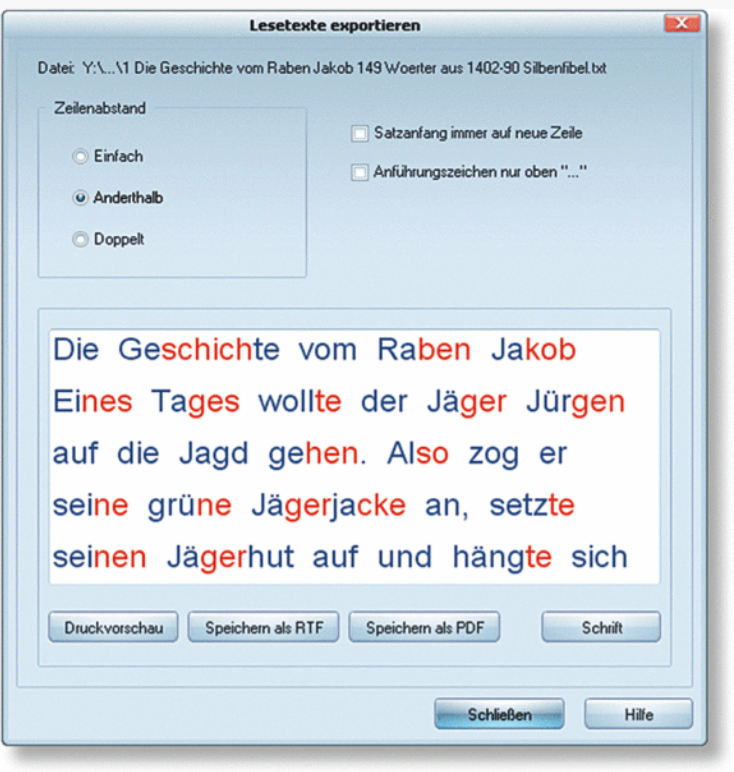
\includegraphics[width=.5\linewidth]{figures/ABCsilbengenerator}
	\caption{Bildschirmfoto des Silbengenerators auf der Internetseite von \textit{ABC der Tiere}\cite{ABCSilbengenerator2018}}
	\label{fig:ABCsilbengenerator}
\end{figure}
Ein weiteres zu erwähnendes Tool ist die \textit{Celeco Druckstation}\cite{celeco2018}. Auch hier können eigene Texte entweder mit farblich markierten Silben oder Silbenbögen gedruckt werden. Das Programm ist zusammen mit der \textit{Celeco} Software (LRS Therapie und Leseübungen) erhältlich, welche für Windows verfügbar ist.

Um die Vorteile durch silben- und betonungsorientiertes Lernen auszunutzen ist man oft auf Materialien von Verlagen oder eine aufwendige manuelle Erstellung von Texten angewiesen. Dies bekräftigt die Motivation eine neue Lösung zu entwickeln um eigenes Übungsmaterial erstellen zu können, was zudem flexibel gestaltbar und z.B. auf bestimmte Schüler anpassbar ist.

\section{Technischer Hintergrund}

Um das Ziel einer automatischen Analyse und Annotation beliebiger Texte zu realisieren, wurden vor Allem die folgenden zwei Schritte untersucht:
\begin{enumerate}
	\item Linguistische Analyse (Zerlegung des Texts in Wörter)
	\item Bestimmung von Silbentrennung und Betonungsmuster
\end{enumerate}

\subsection{Linguistische Analyse}
Da die von der Applikation zu verarbeitende Eingabe ein Text ist, also eine beliebige Folge von alphanumerischen Zeichen, sowie Leerraumzeichen und Interpunktionen, muss diese Eingabe zunächst korrekt in Wörter zerteilt werden. Dieser Schritt wird \textbf{Tokenisierung} genannt. Zusätzlich werden auch von einem \textbf{Tagger} jedem Wort weitere Informationen, wie z.B. die Wortart (\textit{Part-of-Speech-/POS-Tagger}) hinzugefügt. Diese werden üblicherweise mithilfe eines entsprechenden Lexikons nachgeschlagen\cite{Carstensen2004}. Der für dieses Projekt verwendete Parser wird in Abschnitt \ref{sec:spacy} näher beschrieben. Beim Parsen des Texts können folgende wichtige Informationen extrahiert werden:

\begin{itemize}
	\item \textbf{Textstruktur}: Zerlegung des Texts in Tokens, dadurch wird bestimmt, ob es sich bei den Zeichenfolgen um Wörter oder andere Strukturen wie Leerraum oder Interpunktionen handelt.
	
	\item \textbf{Wortart}: Die Werte der Wortart- (\textit{Part-of-Speech-}) Tags geben an um was für ein Wort es sich handelt (mit dem \textit{spacy} Parser z.B. \textit{NOM} für Nomen, \textit{PROPN} für Eigennamen, \textit{DET} für Artikel etc.).
	\item  \textbf{Lemma}: Gibt die Grundform eines Wortes an, welche je nach Wortart unterschiedliche Ausprägungen annehmen kann. Bei Verben steht hier z.B. der Infinitiv, bei Pronomen die erste Person Singular etc.
\end{itemize}

\subsection{Datenbank zur Wortbetonung}
\label{sec:forschung-database}

Liegt der Text als Liste von Wörtern (Tokens) vor, so können weitere Analysen auf dieser Ebene vorgenommen werden. Für die Annotation des Textes muss eine Repräsentation in Silben vorliegen, zusätzlich wird die betonte Silbe im Wort gesucht. Es ist durchaus möglich, dass in einem Wort mehrere Betonungen vorkommen (gerade bei Wortkompositionen, die im Deutschen häufig zu finden sind, z.B. \textit{heraus+kommen}). Dies wird hier vernachlässigt, es wird nur eine Hauptbetonung, die erste vorkommende Betonung im Wort gesucht. Eine weitere Einschränkung die getroffen wurde ist die Beschränkung auf die Annotation der Betonung im Wort-Kontext (und nicht im Zusammenhang des Satzes). Hier wäre es auch denkbar gewesen, für die Erlernung von Sprachrhythmus und Satzmelodie die Betonung über Wortgrenzen hinaus in Sätzen hervorzuheben. Folgen z.B. viele kurze Wörter aufeinander, so werden diese im natürlichen Sprachrhythmus nicht alle gleich betont gesprochen, sondern eine Betonung findet nur in bestimmten Wörtern im Satz statt. Im Rahmen der vorliegenden Arbeit wurde dieser Aspekt der Prosodie vernachlässigt. Das Ziel war es, bei Menschen mit LRS die Dekodierung des Wortbildes mithilfe von Silben zu erleichtern, daher wurde sich auf die Möglichkeit konzentriert, einzelne Silben und die betonte Silbe im Wort hervorzuheben.\\

Informationen zur Worttrennung in Silben und zur Wortbetonung lassen sich in diversen Lexika finden. \todo{Welche: PhonoLex Core mit Balloon, generell Wörterbücher für Silbentrennung, Hyphenator von OpenOffice oder LaTex} Für die weitere Verwendung in der zu entwickelnden Applikation wurde als Grundlage das Lexikon CELEX2 gewählt. Dabei handelt es sich um ein umfangreiches Sprachlexikon für die Sprachen Englisch, Deutsch und Niederländisch. Verarbeitet wurden hier zunächst nur die deutsche Sprache. Neben der gesuchten Worttrennung und -betonung enthält es auch weitere linguistische Informationen wie Wortart und Grundformen, sowie phonologische und orthographische Annotationen \cite{Burnage1990}. \todo{Alternativen, welche? könnten zusätzlich oder anstelle des CELEX verwendet werden. z.b. PhonoLex Core, besser als CELEX, umfangreicher (quelle!), aber nicht kostenfrei}

Weiterführend wurden auch Text-To-Speech Systeme untersucht. Diese generieren bei gegebenem Eingabetext automatisch synthetische Sprache. Dazu wird intern ein phonologisches Modell aufgebaut, um zu funktionieren muss also zwangsweise eine phonologische Analyse durchgeführt werden, welche auch die Wortbetonung bestimmt. Beispielsweise liefern die Systeme MARY TTS\tocite{MARY} oder BAS\tocite{BAS} auch textuell annotierte Formen ihrer phonologischen Analyse, die als Grundlage zur Extraktion von Betonung dienen können.\\

Linguistische Datenbanken können aufgrund des Umfangs und der Flexibilität von Sprachgrammatiken niemals vollständig sein. Es wurde daher ein Weg gesucht die Datenbank auf unkomplizierte Weise erweiterbar zu machen. Dies kann mit einem geeignete User-Interface durch ExpertInnen erfolgen, die unbekannte Einträge ergänzen und hinzufügen. Einige Arbeiten hatten bereits Erfolg damit, solche Aufgaben durch \textit{Croudsourcing} effektiv auch auf Nutzer zu verteilen, die keine ExpertInnen für den jeweiligen Anwendungsbereich sind. Da die zu entwickelte Applikation auch ein Nutzerverwaltungssystem beinhaltet, wurde untersucht, ob Datenbankeinträge mithilfe mehrerer Nicht-Experten NutzerInnen per einfachem Mehrheitsentscheid verifiziert werden können. Weiterführend könnten auf Plattformen wie Amazon Mechanical Turc oder CrowdFlower beispielsweise leicht Arbeiter anonym engagiert werden, die solche Aufgaben erledigen\cite{Snow2008}. Diese Plattformen wurden beispielsweise von Zaidan und Callison-Burch (für automatisierte Übersetzungen)\cite{Zaidan2011} oder De Kuthy, Ziai und Meurers\cite{Meurers2015} (für Fokusannotation) benutzt, um computerlinguistische Aufgaben zu erledigen.
\cleardoublepage

% !TEX root = ../ausarbeitung.tex

\chapter{Anforderungsanalyse und Spezifikation}

Schon während der Konzeption des Projekts ist klar geworden, dass die zu entwickelnde Software eine relativ komplexe Architektur erfordert. Da eine Browser Applikation entwickelt wurde, musste die Software in Teilprojekte untergliedert werden. Zum einen das User-Interface für die Web Applikation und zum Anderen die Programmlogik, welche auf Grund der benötigten Funktionalitäten (wie Datenbankanbindung und Algorithmen zur Textverarbeitung) nicht sinnvoll im Web Client implementiert werden konnte.\\
Um eine Spezifikation für die Software zu entwerfen und den zu verwendenden Software-Stack zu definieren, wurde zunächst eine Anforderungsanalyse durchgeführt, die im Folgendem Teil beschrieben wird. Im darauffolgenden Kapitel gehe ich Schritt für Schritt auf die Entwicklung des Gesamtsystems ein.

\section{Anforderungen an die Software}

Zunächst wurde festgestellt, welche Funktionen die App dem Nutzer bieten soll. Dazu wurden Folgende mögliche Szenarien aufgestellt:

\paragraph{Text Analyse} 
Der User möchte einen Fließtext eingeben und von der Anwendung annotieren lassen. Nach der Eingabe soll das Ergebnis annotiert in der App dargestellt werden.

\paragraph{Anpassung der annotierten Darstellung}
Der User möchte die Parameter des annotierten Texts ändern. Angepasst werden können sollen die Texteigenschaften (Font, Zeilenabstand, Zeichenabstand) und die Darstellung der Annotation (Farben für betonte und unbetonte Silbe, Silbenabstand, Trennzeichen zwischen Silben)

\paragraph{Export der annotierten Darstellung}
Der User hat die Möglichkeit verschiedene Formate des annotierten Texts zu exportieren, z.B. Druck, HTML oder Word.

\paragraph{Verwaltung von User Accounts}
Dem User soll die Möglichkeit gegeben werden, einen User Account zu erstellen um persönlich verwendete Daten (z.B. Texte oder Wortsegmentierungen) speichern zu können. Dazu werden Funktionen und Interfaces zur Registrierung eines Nutzeraccounts, Login, Logout, zum Bearbeiten der Nutzerinformationen und zum Löschen des Accounts bereitgestellt.

\paragraph{Behandlung unbekannter Wörter}
Der Nutzer kann nacheinander die Segmentierung von Wörtern, die durch das System nicht eindeutig bestimmt wurden konnten, selbst manuell festlegen.

\paragraph{Bestimmung der Segmentierung unbekannter Wörter}
Für ein unbekanntes Wort wählt der User in einem neuen View die Segmentierung selbst aus. Dafür werden folgende Möglichkeiten gegeben:
\begin{itemize}
	\item Input aus G2P Systemen wie MARY TTS
	\item Manuelle Segmentierung mit geeignetem User Interface
	\item Eventuell weitere Quellen für die Segmentierung (z.B. Duden)
\end{itemize}

\paragraph{Speicherung von Nutzer Segmentierungen}
Vom Nutzer hinzugefügte Segmentierungen sollen (lokal für diesen Nutzer) gespeichert werden können und beim nächsten Vorkommen in einem Text automatisch verwendet werden.

\paragraph{Speicherung und Wiederverwendung von Annotationskonfigurationen für Texte}
Die Einstellungen, die ein Nutzer an einenm annotierten Text vorgenommen hat, können als Vorlage für andere Texte gespeichert werden. In den Annotationseinstellungen eines Textes kann eine zuvor gespeicherte Konfiguration wiederverwendet werden.

\paragraph{Speicherung und Wiederverwendung von Nutzertexten}
Analysierte Texte können vom Nutzer zusammen mit der verwendeten Konfiguration gespeichert werden. Den Texten können Metadaten zugeordnet werden, z.B. Thema, Niveau, Zielgruppe. Im Benutzerbereich werden die Texte, die der Nutzer hinzugefügt hat, geeignet strukturiert, dargestellt. Dem Nutzer wird die Möglichkeit gegeben, den gespeicherten Text erneut analysieren zu lassen.

\paragraph{Verifizierung unbekannter Wörter}
Manuelle Segmentierungen von unbekannten Wörtern müssen auf Korrektheit überprüft werden. Dazu wird jeder Nutzer aufgefordert, die Einträge anderer Nutzer zu überprüfen. In einem View, ähnlich zur manuellen Segmentierung, kann der Nutzer Einträge anderer Nutzer bestätigen oder Gegenvorschläge übermitteln.

\paragraph{Expertennutzer}
Ein Experte (z.B. Linguist oder Lerntherapeut) kann sich als solcher bei der Erstellung eines Accounts identifizieren. Bei der Wort Verifizierung zählt die Stimme der Expertennutzers mehr als die eines Nutzers, der kein Experte ist.

\subsubsection{User Interface}
Von diesen Szenarien ausgehend wurde in den Folgenden Schritten ein geeignetes User Interface erarbeitet:

\paragraph{Informationsstruktur}
\todo{information structure, menü hierarchie, aufbau des user interfaces (links, lineare hierarchie), storyboards}\\

\paragraph{Farbschema}
\todo{color scheme https://color.adobe.com}

\subsection*{Grundlegende Anforderungen}

Aus den oben beschriebenen Use Cases lassen sich diverse Anforderungen an die Software spezifizieren:

\begin{itemize}
	\item Service zur Textanalyse
	\item Wortdatenbank
	\item Service zur Manipulation der Wortdatenbank
	\item Service zur Nutzerverwaltung
	\item Speicherung Nutzer spezifischer Daten
	\item Geeignetes User Interface zur Darstellung von Texten und zur Interaktion mit dem System
\end{itemize}




\section{Softwarestack}

Bei der Vielseitigkeit der verschiedenen Anforderungen ist die Wahl der zu verwendenden Technologien nicht unerheblich. Programmiersprachen und Frameworks müssen sorgfältig ausgewählt werden um für jedes Teilproblem eine passende Lösung zu entwickeln.\\
Die erste wichtige Unterteilung fand statt zum Einen in ein Frontend welches die zum Benutzer darstellt und zum Anderen in ein Backend welches die vom System verwendeten Daten speichert und manipuliert und diese mit Hilfe geeigneter Algorithmen an das Frontend schickt. Eine genaue Beschreibung über den detaillierten Aufbau und die Funktion von Front- und Backend wird in Kapitel 4 gegeben.\\

\todo{kleine Grafik zu front backend}

Diese Aufteilung ist in der Webentwicklung weit verbreitet \tocite{front backend} und bietet einige Vorteile gegenüber eins komplett integriertem Gesamtsystems:

\begin{itemize}
	\item Klare Trennung von Darstellung und Datenverarbeitung
	\item Einfachere Fehlersuche durch kleinere Komponenten
	\item Bei der Entwickelung zusätzlicher Frontends (z.B. für Android oder iOS) muss nur ein neuer Teil des Softwaresystems entwickelt werden, während das Backend gleich bleibt
	\item Einfache Arbeitsaufteilung im Entwicklerteam (relevant bei Weiterentwicklung der Anwendung mit mehreren Personen)
	\item \todo{more?}
\end{itemize}

\subsection{Verwendete Technologien}
Für verschiedene zu realisierende Ziele gibt es für jedes Teilziel Technologien, die Vorteile gegenüber anderen bieten. Die Verwaltung von Datenbanken ist zum Beispiel besser mit einer Server seitigen Skriptsprache zu implementieren, als mit den Möglichkeiten, die das Frontend bietet. Im Web Frontend dagegen sind gewisse Technologien wie HTML, CSS und JavaScript standard, die zwangsläufig verwendet werden müssen. Daher wird In der Applikation eine Vielzahl verschiedener Technologien verwendet, eine Übersicht ist hier gegeben:

\begin{itemize}
	\item Backend: python, REST API, sowie die python Frameworks flask, spacy und sqlalchemy
	\item Frontend: HTML, CSS, JavaScript, AngularDart
	\item Kommunikation mit JSON
	\item Deployment mit Apache auf AWS Server
\end{itemize}

Im Folgenden werden die einzelnen Technologien und deren Vorteile beschrieben.

\subsection{Backend}
Backend as a service: e.g. Firebase, zu unflexibel\\

welche alternativen fuer backend\\
frontend unabhäng von daten

\subsubsection{python}
warum python\\
flexibel und schnell, viele frameworks\\
Requests an externe Services, MARY, BALLOON

\subsubsection{REST API}
was? warum?

\subsubsection{flask}
gutes framework für REST

\subsubsection{spacy}
parser, alternative NLTK, auch benutzt, warum ist spacy besser?\\
tokenizer, part of speech

\subsection{Frontend}

webapplication, html css, single-view-application, dynamic data loading
viele frameworks, verwende AngularDart
no javascript: weakly typed languages transforming to JS: GWT (java), typescript, Dart

\subsubsection{Angular Dart}
warum? javascript is bad.\\

data binding\\
more lightweight vs Java\\

many google apps use it\\
objektorientierung\\

angular? angular2?\\

dart, google\\
alternativen, typescript...\\

dart2js compiler, wie funktioniert dieser\\

\subsection{Deployment}

webserver für frontend, auf eigenem server mit apache gehostet\\
flask python service läuft immer, REST schnittstelle\\






%-----------------------------------------------------------------------------------------
%-----------------------------------------------------------------------------------------

\cleardoublepage

% !TEX root = ../ausarbeitung.tex

\chapter{Entwicklung der Anwendung}

Im Rahmen der Masterarbeit wurde die beschriebende Web Applikation prototypisch entwickelt. Die dazu nötige Planung und die verwendeten Technologien wurden in den vorherigen Kapiteln geschildert. Nun wird auf den Prozess der Entwicklung und auf die detaillierte Struktur der Applikation eingegangen.\\

Das Entwicklung des Systems wurde in drei Teilprojekte untergliedert:
\begin{enumerate}
	\item Erstellung der Basisdatenbank aus dem Wörterbuch CELEX2
	\item Entwicklung des Backends mit python
	\item Entwicklund des Frontends mit gängigen Webtechnologien und AngularDart
\end{enumerate}

Dabei wurde Schritt 1 als Erstes durchgeführt, die Verfügbarkeit der Basisdatenbank war Voraussetzung um mit der Entwicklung von Front- und Backend zu beginnen. Als eine erste Version der Datenbank vorlag, wurde zunächst mit der Entwicklung eines minimalen Backends begonnen, welches die Kernfunktionalität - das Analysieren von Texten - beherrschte. Damit konnte eine erste Version des Frontends erstellt werden, um einen ersten Eindruck zu bekommen, wie alle Technologien miteinander funktionieren.\\
Im Anschluss konnten Front- und Backend parallel entwickelt werden. Es wurden immer wieder Funktionen im Backend entwickelt, woraufhin das Frontend angepasst wurde, um dem Nutzer diese Funktionen anzubieten. Zu diesem Zeitpunkt wurde auch die Basisdatenbank einige male überarbeitet, so ist das Gesamtsystem Schritt für Schritt auf eine agile Weise \tocite{agil} gewachsen. Im Folgenden wird näher auf die drei Teilprojekte eingegangen.

\section{Erstellung einer Basisdatenbank}
\label{sec:worddatabase}

Für die Segmentierung von Wörtern in Silben mit Betonung wird eine sqlite Datenbank verwendet, deren Entwicklung hier beschrieben wird. Als Grundlage für die Datenbank dient das digitale Lexikon \todo{Lexikon/woerterbuch...?} CELEX2, wie in Kapitel \ref{sec:forschung-database} beschrieben. Folgende Informationen wurden dem CELEX entnommen und in der Datenbank gespeichert:

\paragraph{Worttext}
Hier wurde darauf geachtet, eine einheitliche orthographische Form der Wörter durchzusetzen. Wörter bestehen nur aus Kleinbuchstaben (auch die Anfänge von Nomen und Eigennamen). Außerdem wird hier auf Umlaute verzichtet, \qq{ä} wird durch \qq{ae} ersetzt, \qq{ö} durch \qq{oe}, \qq{ü} durch \qq{ue} und \qq{ß} durch \qq{ss}. Beispielsweise wird das Wort \textit{Häuser} zu \textit{haeuser}. So kann beim Nachschlagen garantiert werden, dass ein Wort nicht wegen uneinheitlicher Schreibweise nicht gefunden wird, sofern alle Umlaute vorher ersetzt wurden.

\paragraph{Wortart}
Um Doppeldeutigkeit zu vermeiden wird ein Eintrag nur eindeutig über das Paar aus Worttext und Wortart identifiziert. Viele Grundformen von Verben kommen zum Beispiel auch als Nomen vor, werden aber dann groß geschrieben (\qq{sie sollte die Maschine \textit{verwenden}} gegen \qq{das \textit{Verwenden} der Maschine}). Die Bezeichner für Wortart sind in verschiedenen Systemen wie dem CELEX und dem NLP parser \textit{spacy} unterschiedlich, daher wird hier eine eigene - im Gesamtsystem konsistente - Benennung der Wortart eingeführt (die Benennung orientiert sich an den Tag Namen des spacy parsers, verwendet jedoch zur Unterscheidung Klein- statt Großschreibung):

\begin{table}[h!]
	\centering
	\begin{tabular}{|l|l|}
		\hline
		Wortart & Benennung/Tag \\
		\hline
		\hline
		Nomen & \textit{noun}\\
		Eigenname & \textit{propn}\\
		Verb & \textit{verb}\\
		Hilfsverb & \textit{aux}\\
		Adjektiv & \textit{adj}\\
		Adverb & \textit{adv}\\
		Artikel & \textit{det}\\
		Adposition & \textit{adp}\\
		Pronomen & \textit{propn}\\
		Konjunktion & \textit{conj}\\
		Zahl & \textit{num}\\
		Partikel & \textit{part}\\
		Zahl & \textit{num}\\
		\hline
	\end{tabular}
	\caption{Benennung der Wortarten in der Applikation}
\end{table}

\paragraph{Silbentrennung}
Die Silbentrennung enthält die einzelnen Silben, getrennt durch einen Querstrich (\qq{-}). Im Gegensatz zum Worttext erhält dieser Eintrag Groß- und Kleinschreibung, sowie alle Umlaute. Die Silbentrennung des Wortes \textit{Möglichkeit} ist also \textit{Mög-lich-keit}.

\paragraph{Betonungsmuster}
Das Betonungsmuster identifiziert eine Silbe als Hauptbetonung im Wort. Dieser Eintrag ist ein String aus aneinandergereihten \qq{0} und \qq{1} Werten. Die \qq{1} bezeichnet dabei die betonte Silbe, die \qq{0} stellt eine unbetonte Silbe dar. Nebenbetonungen werden im Rahmen dieser Arbeit vernachlässigt. Das Betonungsmuster besteht nur aus einer einzigen \qq{1} - der Hauptbetonung - während alle anderen Silben unbetont (\qq{0}) bleiben. Beispiel resultiert das Wort \textit{hervorragend} mit der Silbentrennung \textit{her-vor-ra-gend} in das Betonungsmuster \qq{0100}.

\paragraph{Lemma}
\todo{was genau? auch im celex, keine wirkliche anwendung in der app, vielleicht ausblick}

Neben den Worteinträgen sollen in der Datenbank noch Informationen über die Herkunft der Wörter gespeichert werden. Neben den Basiseinträgen, die aus dem CELEX extrahiert werden, wird den Nutzern später die Möglichkeit gegeben Einträge zur Datenbank hinzuzufügen. Um diesen Vorgang nachvollziehbar zu machen gibt es eine zweite Tabelle, in welcher Einträge für neu hinzugefügte Wörter mit Zeitstempel angelegt werden. Das Folgende Schema \ref{fig:worddatabase} zeigt die Struktur der Wortdatenbank.

\begin{figure}[h!]
	\centering
	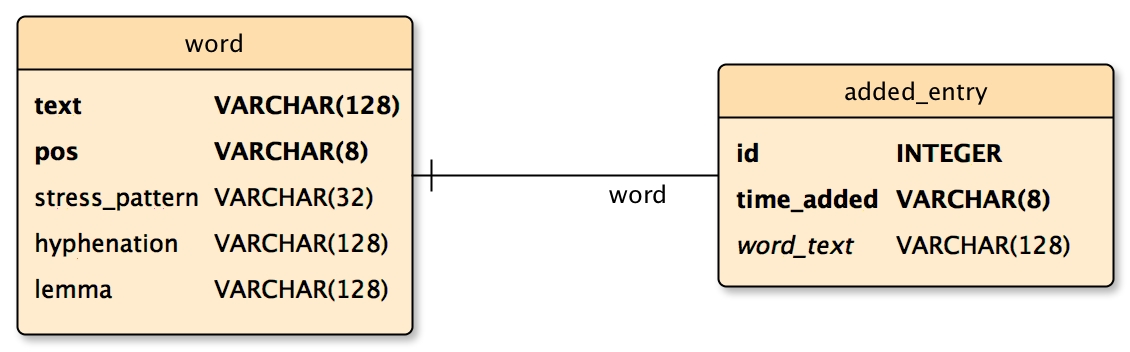
\includegraphics[width=.6\linewidth]{figures/worddb}
	\caption{Schema der Wortdatenbank (\textit{word.db})}
	\label{fig:worddatabase}
\end{figure}

Alle in der Worttabelle beschriebenen Einträge sind auch im CELEX vorhanden. Der Folgende Abschnitt beschreibt, wie die Daten aus dem Lexikon extrahiert und in der Wortdatenbank gespeichert wurden.

\subsection{Implementierung}

Für die Generierung der Datenbank wurde das python Projekt \textit{celex2db} erstellt, welches in \qq{/backend/celex2db} zu finden ist (alle Pfadangaben in diesem Abschnitt beziehen sich auf dieses Verzeichnis). Die Daten im CELEX \todo{in Forschungsstand teil verschieben} sind über mehrere Dateien verteilt. So gibt es eine Teilung in Sprachen (für die Datenbank werden nur Deutsche Wörter benutzt, zu finden in \qq{celex2/german}), Wörter und Lemmata sowie in Orthographie, Phonologie und Morphologie. Die Teilung in Wort und Lemma spart Speicherplatz. Das Lemma eines Verbs, zum Beispiel, ist die Grundform dieses. Zur Beugung \textit{gehst} gehört also das Lemma \textit{gehen}. Viele Eigenschaften des Verbs \textit{gehen} beziehen sich auf alle Flexionsformen, so müssen diese nicht für alle Verbformen redundant gespeichert werden.\\
Die Einträge in den Wortlisten des CELEX verweisen jeweils mit einer ID auf den zugehörigen Eintrag in der Lemma Liste. Da in der zu entwickelnden Datenbank auch das Lemma gespeichert werden soll, müssen sowohl Wort Listen als auch Lemma Listen geparsed werden.\\

Das Hauptskript \qq{celex2db.py} führt die folgenden Schritte aus:
\begin{enumerate}
	\item Parsen der orthographischen Lemma Liste
	\item Parsen der orthographischen und phonologischen Wort Listen
	\item Generierung von Einträgen aus Wort und Lemma Listen und Schreiben in die Datenbank
\end{enumerate}
Während der Ausführung des Skripts werden Schrittweise Fortschrittsangaben mit Fehlern ausgegeben (Schrittweite im Skript einstellbar), da das Parsen und Erstellen der Datenbank einige Zeit benötigt (mehr dazu im Abschnitt \ref{sec:database-results}).

Die Klasse \texttt{CelexDictionary} im Skript \qq{celex.py} bietet die Methoden zum Parsen der Wort und Lemma Listen. Die Struktur ist in \ref{fig:celex2db} dargestellt.\\

\begin{figure}
	\centering
	\todo{Klassendiagramm CelexDictionary}
	\caption{Diagramm der \textit{celex2db} Klassen}
	\label{fig:celex2db}
\end{figure}

In der \texttt{parseLemma} Methode wird die CELEX Datei \qq{gml.cd} verarbeitet. Die morphologische Informationen zu den Lemmata enthält. Jede Zeile enthält ein Lemma, für welches in der Struktur \texttt{CelexLemma} die ID des Lemmas, Text und Wortart gespeichert werden.\\

In der \texttt{parseWords} Methode werden nun die beiden Dateien \qq{g\textbf{p}w.cd} und \qq{g\textbf{o}w.cd} verarbeitet, welche phonologische und orthographische Informationen zu allen enthaltenen Beugungen der Wörter enthalten. Die IDs und Reihenfolge in beiden Wortlisten stimmen überein, sodass beide Listen gleichzeitig verarbeitet werden können. Aus der phonologischen Liste werden der Text des Wortes, der Verweis auf das zugehörige Lemma (lemma\_id) sowie die phonologische Darstellung entnommen. Die orthographischen Liste liefert lediglich die Silbentrennung.\\
Danach wird in der zuvor verarbeiteten Liste der Lemmas, mithilfe der \texttt{lemma\_id} der Text passende Lemmas gesucht und alle verfügbaren Daten in der Struktur \texttt{CelexWord} gespeichert. Die Hauptklasse \texttt{CelexDictionary} enthält ein python Dictionary aller \texttt{CelexWord} Einträge, siehe Abbildung \ref{fig:celex2db}.

Letztendlich werden die Einträge der Wortliste im Skript \qq{writeSQLite.py} in die Datenbank übertragen. In einem frühen Entwicklungsstadium wurden hier SQL Instruktionen verwendet um die Datenbankeinträge zu erstellen. Nach der Entwicklung des \texttt{DictionaryService} im Backend (genauer beschrieben im Abschnitt \ref{sec:dictionary-service}wurde später direkt auf diesen zugegriffen, um Redundanten Code zu vermeiden. Ein einfacher Funktionsaufruf der Methode \texttt{add\_word} des \texttt{DictionaryService} fügt den Eintrag der Wortdatenbank hinzu.

\subsection{Ergebnisse}
\label{sec:database-results}

Ein Wort soll eindeutig identifizierbar sein durch den Worttext und die Wortart. Daher wurde in der Datenbank die Kombination der Felder \textit{text} und \textit{pos} (part of speech/Wortart) als Primärschlüssel gewählt. Ein doppeltes Einfügen eines Wortes in die Datenbank verletzt den SQL \textit{UNIQUE Constraint}, und ist somit nicht möglich. Die dadurch von python geworfene Exception wird in diesem Fall abgefangen und und die \texttt{add\_word} Methode liefert \texttt{None} zurück.\\
Trotz der Wortidentifizierung anhand von zwei Merkmalen, beinhaltet der CELEX teilweise redundante Informationen. 4 356 Einträge verursachen aufgrund des \textit{UNIQUE Constraint} Fehler, da sie mit gleichem Text und gleicher Wortart schon in der Datenbank waren, diese wurden somit übersprungen. Bei einem kompletten Neuaufbau der Datenbank aus dem CELEX werden 360 243 Wörter hinzugefügt. Die Datenbank wurde als sqlite Datei \qq{/backend/db/words.db} angelegt.

\section{Backend}
\label{sec:etwicklung-backend}
Das in python mit dem Web-Framework flask entwickelte Backend verarbeitet sämtliche, vom Frontend gesendeten HTTP requests. Es sendet entweder eine Antwort mit den geforderten Daten oder einen HTTP Fehlercode mit Fehlermeldung. Das Backend Projekt befindet sich in \qq{/backend/API}. Es wurde in die drei Services \textit{DictionaryService}, \textit{UserService} und \textit{VerificationService} strukturiert. Das Hauptsript \todo{rename} \qq{LinguisticTextAnnotation.py} verwaltet diese Services, startet die flask Applikation und definiert die einzelnen Routen für HTTP requests (diese werden im folgenden Abschnitt aufgelistet). Folgende Grafik zeigt eine Übersicht über die Struktur des Backends.

\todo{Grafik Backend}

\subsection{HTTP Routen}
Tabelle \ref{table:backendroutes} bietet eine Übersicht über die verfügbaren Routen, welche die HTTP requests verarbeiten. Zudem werden kurz der Zweck und die Parameter der Route beschrieben. Ein \textit{X} in der Spalte Authentifizierung bedeutet, dass die Mail Adresse und das Passwort des Nutzers übergeben werden muss. Diese werden nicht extra in der Spalte Parameter aufgeführt (außer in der \qq{/user/authenticate} Route, diese dient ausschließlich dazu, die Übermittelten Nutzer Credentials zu prüfen).

\begin{table}[h!]
	\centering
	\begin{tabular}{|l|l|l|c|}
		\hline
		\textbf{Route} & \textbf{Parameter} & \textbf{Methode} & \textbf{Auth.}\\
		\hline
		\hline
		/query/word & text, pos & GET & \\
		\hline
		/query/text & text & POST & \\
		\hline
		/query/segmentation& word & GET & \\
		\hline
		\hline
		/user/register & email, password, & POST & \\
		& first\_name, last\_name, is\_expert &&\\
		\hline
		/user/authenticate & \textit{email, password} & POST & X\\
		\hline
		/user/delete & id & POST & X\\
		\hline
		\hline
		/user/word/add& text, stress\_pattern, hyphenation, pos & POST & X\\
		\hline
		/user/word/delete& id & POST & X\\
		\hline
		/user/word/list & - & POST & X\\
		\hline
		\hline
		/user/configuration/add & name, \textit{options} & POST & X\\
		\hline
		/user/configuration/update & id, name, \textit{options}  & POST & X\\
		\hline
		/user/configuration/list & - & POST & X\\
		\hline
		/user/configuration/delete & id & POST & X\\
		\hline
		\hline
		/user/text/add & title, text & POST & X\\
		\hline
		/user/text/delete & id & POST & X\\
		\hline
		/user/text/list & - & POST & X\\
		\hline
		\hline
		/user/verification/query & - & POST & X\\
		\hline
		/user/verification/submit & id, stress\_pattern, hyphenation & POST & X\\
		\hline
	\end{tabular}
	\caption{Backend routen für HTTP requests mit Parametern und Methode}
	\label{table:backendroutes}
\end{table}

Die bei \qq{user/configuration/} nicht aufgeführten \textit{options} bestehen aus allen für die Annotationsvorlage gespeicherten einstellungen. Dies sind die Folgenden Felder: \textit{stressed\_color, unstressed\_color, word\_background, alternate\_color, syllable\_separator, line\_height, word\_distance, syllable\_distance, font\_size, letter\_spacing, use\_background, highlight\_foreground, stressed\_bold, use\_alternate\_color, use\_syllable\_separator, part\_of\_speech\_configuration}.

\subsection{Dictionary Service}
\label{sec:dictionary-service}

Das Modul \textit{DictionaryService.py} verarbeitet Anfragen zur Textanalyse, verwaltet die Wortdatenbank und generiert Vorschläge für die manuelle Segmentierung von Wörtern. Das Schema der Wortdatenbank zeigt Abbildung \ref{fig:worddatabase}. Folgende Klassen werden definiert:
\begin{itemize}
	\item \texttt{Word}: Entspricht Tabelle \textit{word} in der Wortdatenbank (Abbildung \ref{fig:worddatabase}) und speichert die Merkmale eines Wortes.
	\item \texttt{AddedEntry}: Enthält einen Verweis (Fremdschlüssel) auf ein hinzugefügtes Wort und dessen Erstellungszeitpunkt.
	\item \texttt{Segmentation}: Modelliert einen Segmentierungsvorschlag. Die Klasse enthält Worttext, Segmentierung und Betonungsmuster. Außerdem speichert sie den Namen (\texttt{origin}) und die Herkunft (\texttt{source}) der Quelle des Vorschlags (z.B. MARY TTS).
\end{itemize}

Im Folgenden werden die Funktionen des \textit{DictionaryService} genauer beschrieben.

\subsubsection{Funktionen der Wortdatenbank}
\begin{itemize}
	\item Die Methode \texttt{add\_word} bekommt Worttext, Betonungsmuster, Wortteilung, Lemma und Wortart übergeben (s. Abschnitt \ref{sec:worddatabase}), fügt das Wort der Datenbank hinzu und liefert eine \texttt{Word} Instanz zurück. Im Falle eines Fehlers oder falls das Wort schon existiert, gibt die Methode \texttt{None} zurück.
	
	\item \texttt{query\_word} schlägt ein Wort mit den Parametern Worttext und Wortart in der Datenbank nach und gibt das annotierte Wort im JSON (\textit{text}, \textit{stress\_pattern}, \textit{hyphenation}, \textit{lemma}, \textit{pos}) Format zurück. Als Parameter kann optional der eingeloggte Nutzer übergeben werden. Ist das der Fall, wird zuerst überprüft, ob im Nutzeraccount (s. Abschnitt \ref{sec:userservice}) eine manuelle Segmentierung für das Wort gespeichert ist und falls ja, diese zurückgegeben. Werden in der Wortdatenbank mehrere Wörter gefunden, die dem gesuchten Worttext entsprechen, wird zusätzlich die Wortart geprüft und der passende Eintrag (bzw. der Erste Eintrag, falls kein Wort mit der entsprechenden Wortart gefunden wird) zurückgegeben.
	
\subsubsection{Textanalyse}
Die Methode \texttt{query\_text} bekommt den gesamten zu analysierenden Text übergeben (sowie optional den eingeloggten Nutzer für manuelle Worteinträge). Der Text wird zunächst mit dem spacy Parser analysiert. Dieser zerlegt den Text in einzelne Wörter und Trennzeichen und gibt eine Liste von Tokens zurück. Nun wird über die Liste der Tokens iteriert und dabei wiederum eine Liste von JSON Einträgen generiert, welche am Schluss von der Methode zurückgegeben wird. Jedes spacy Token liefert den Worttext \texttt{text} die Wortart \texttt{pos\_} und das Lemma \texttt{lemma\_}. Das Token wird wie folgt verarbeitet:

\begin{enumerate}
	\item In jedem Fall wird ein neuer JSON Eintrag angelegt und die Felder \texttt{text}, \texttt{pos} und \texttt{lemma} mit den entsprechenden Inhalt des spacy Tokens gefüllt.
	
	\item Enthält der Worttext einen Linebreak \qq{\texttt{\textbackslash n}}, so wird das JSON Feld \texttt{type} mit \textit{linebreak} belegt.
	
	\item Enthält der Worttext einen Trennstrich \qq{\texttt{-}}, so handelt es sich um ein zusammengesetztes Wort (z.B. \textit{100-Millionen-Einwohner-Staat}). Hier werden alle Trennstriche durch Leerzeichen ersetzt. Der resultierende String wird dann erneut mit spacy analysiert und die Tokens dann entsprechend verarbeitet. Hinter jedem Teilwort (außer dem Letzten) wird manuell der Trennstrich als eigenes Token eingefügt.
	
	\item Entspricht der Wortart-Tag einem String aus \texttt{['X',} \texttt{'PUNCT', }\texttt{'NUM', }\\
	\texttt{'SPACE']}, so handelt es sich um eine dem Parser unbekannte Zeichenfolge, eine Zahl, ein Satz- oder Leerzeichen. Diese Tags werden nicht nachgeschlagen sondern mit dem JSON \texttt{type} Feld \textit{ignored} der Rückgabeliste hinzugefügt.
	
	\item Trifft keiner dieser Sonderfälle zu, wird das Wort mit der Methode \texttt{query\_word} nachgeschlagen. Wird dieses gefunden (Rückgabewert nicht \texttt{None}), wird der \texttt{type} auf \textit{annotated\_word} gesetzt. Das JSON Feld \texttt{annotation} enthält dann die Informationen des annotierten Wortes (von \texttt{query\_word} zurückgegeben). Ist das Wort nicht in der Datenbank, so enthält das Feld \texttt{type} den Wert \textit{not\_found}.
\end{enumerate}

\end{itemize}

\subsubsection{Generierung von Segmentierungsvorschlägen}
\label{sec:segmentation-proposals}

Der \texttt{DictionaryService} bietet auch die Möglichkeit, automatisch Segmentierungsvorschläge zu generieren. Diese werden im Frontend dazu benutzt, den NutzerInnen bei der manuellen Wortsegmentierung die Arbeit zu erleichtern, indem das Wort schon in Silben zerlegt wird und versucht wird, automatisch die Wortbetonung zu bestimmen. Der Standardvorschlag, den das System liefert ist einfach die Silbentrennung, die der Python Silbentrenner \textit{Pyphen} liefert. Diese ist in vielen Fällen korrekt und bietet in jedm Fall einen Anhaltspunkt für die Silbentrennung des Wortes. Zudem wird beim Standardvorschlag ein Betonungsmuster generiert, welches immer die erste Silbe im Wort betont. Auch das ist in der Deutschen Sprache oft der Fall, so können Betonung und Silbentrennung bei der manuellen Analyse einfach bestätigt werden.\\

Bei der Abfrage der Vorschläge im Backend wird eine Liste von Segmentierungsvorschlägen zurückgeliefert. Der Standardvorschlag mit \textit{Pyphen} ist nur eine Möglichkeit. Hier wurde überlegt, aus mehreren externen Systemen, wie z.B. MARY TTS oder BAS (s. Abschnitt \ref{sec:forschung-database}), oder später auch z.B. Duden und Anderen, Vorschläge zu sammeln und den NutzerInnen in einer Liste zu präsentieren, aus der der passendste Vorschlag ausgewählt werden kann. Exemplarisch wurde hier eine Anfrage an MARY TTS geschickt und in der Antwort an das Frontend mit eingebunden. Das System kann ebenfalls mit HTTP Requests abgefragt werden. Das entsprechende Interface ist unter \textit{http://mary.dfki.de:59125/process} zu finden. Tabelle \ref{table:mary} zeigt die bei der Anfrage verwendeten GET Parameter. MARY liefert eine Antwort im XML Format zurück, die die phonologische Silbentrennung und die Betonung enthält. Das XML wird entsprechend geparsed, womit dann ein neuer Segmentierungsvorschlag bestimmt werden kann.

\begin{table}[h!]
	\centering
	\begin{tabular}{|l|l|}
		\hline
		\textbf{Parameter} & \textbf{Wert}\\
		\hline
		\hline
		INPUT\_TEXT & \textit{das abzufragende Wort}\\
		INPUT\_TYPE & TEXT\\
		OUTPUT\_TYPE & ACOUSTPARAMS\\
		LOCALE & de\\
		\hline
	\end{tabular}
	\caption{GET Parameter für Anfrage an MARY TTS}
	\label{table:mary}
\end{table}

\subsection{User Service}
\label{sec:userservice}

Der \texttt{UserService} dient der Verwaltung der Nutzerdaten und der Authentifizierung. Nutzerkonten bestehen aus Email Adresse, Passwort und Vor- und Nachnamen der Nutzerin oder des Nutzers. Daneben werden die Resourcen \textit{user\_text}, \textit{user\_word}, \textit{text\_config} und \textit{pos\_config} verwaltet. Welche Funktionen für die jeweilige Ressource zur Verfügung stehen, wird im Folgenden erklärt. Abbildung \ref{fig:userdb} zeigt das Schema der Nutzerdatenbank.

\begin{figure}[h!]
	\centering
	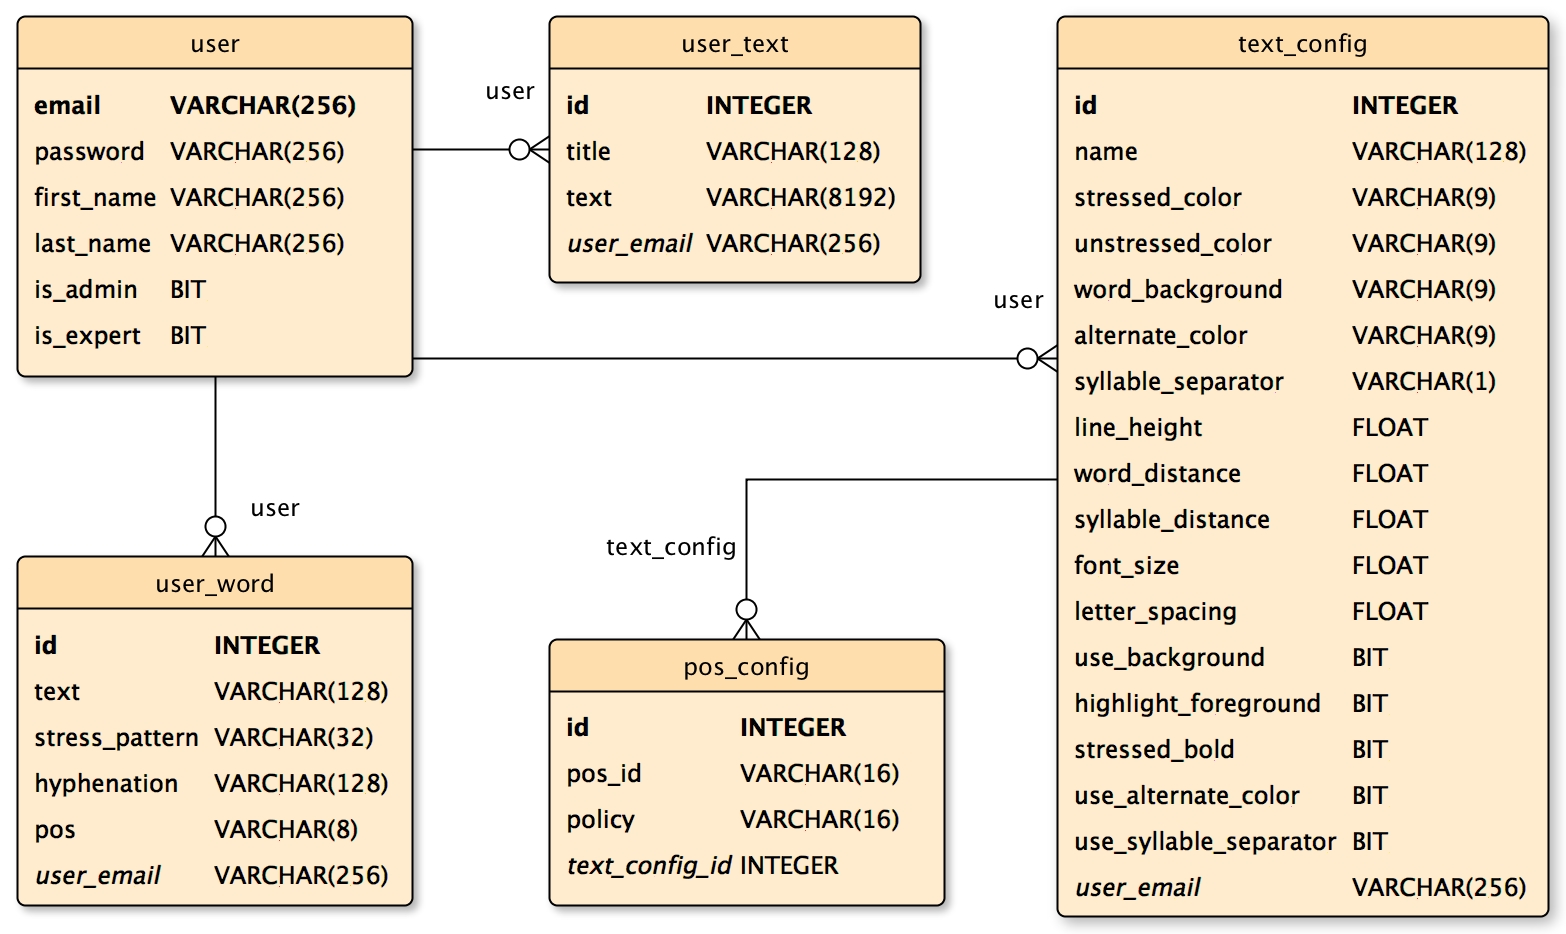
\includegraphics[width=.8\linewidth]{figures/userservicedb}
	\caption{Schema der User Datenbank (\textit{user.db})}
	\label{fig:userdb}
\end{figure}

\begin{itemize}
	\item Zur \textbf{Authentifizierung} wird überprüft, ob ein Nutzerkonto für die als Parameter übergebene Email Adresse und das übermittelte Passwort existiert.
	
	\item \textbf{Nutzertexte} (\textit{user\_text}) können mit Text und Titel erstellt, sowie mit entsprechenden Anfragen abgefragt (als Liste aller Texte eines Nutzerkontos) oder entfernt werden.
	
	\item Auch für \textbf{Nutzerwörter} (\textit{user\_word}, Einträge, die durch die manuelle Segmentierung entstehen), können mit Text, Silbentrennung, Betonungsmuster und optional Wortart angelegt, sowie abgefragt (ebenfalls als Liste aller Wörter eines Nutzerkontos) oder gelöscht werden.
	
	\item Für \textbf{Annotationskonfigurationen} (\textit{text\_config}) gibt es vier Funktionen: Sie können als Liste abgefragt oder mit der zugehörigen \textit{id} gelöscht werden, sowie angelegt und aktualisiert werden. Beim Anlegen und Aktualisieren werden sämtliche Attribute der Konfiguration (Name, Silbenfarben, Texteinstellungen, wie Silben- oder Wortabstand etc.) in der Anfrage mit übergeben. Auch die Konfigurationsliste für die Wortarten (\textit{pos\_config}), die für jede Wortart die Einstellung, ob diese annotiert oder ignoriert wird speichert, wird in der Anfrage benötigt.
\end{itemize}


\subsection{Verification Service}
\label{sec:verification-service}

Von den NutzerInnen manuell erstellte Segmentierungen für Wörter können nicht direkt in die globale Wortdatenbank für alle Nutzer übernommen werden, da bei der Segmentierung Fehler gemacht werden können. Der \texttt{VerificationService} definiert die Funktionen mit denen zu verifizierende Segmentierungen abgefragt oder Verifizierungsvorschläge abgeschickt werden können.\\
Ein zu verifizierender Eintrag ist hierbei direkt ein \textit{user\_word} (s. Abbildung \ref{fig:userdb}), dass von einer Nutzerin oder einem Nutzer bei der manuellen Segmentierung erstellt wurde. Die Verifizierung (Klasse \texttt{VerificationProposal}) bezieht sich auf diesen Eintrag und enthält ebenfalls Silbentrennung und Betonungsmuster für das Wort. Nach der Übermittlung eines Verifizierungsvorschlags prüft ein Algorithmus, ob ausreichend Verifizierungen unterschiedlicher NutzerInnen für das Wort übereinstimmen (also Silbentrennung und Betonung identisch sind). Ist dies der Fall, wird das Wort in die globale Wortdatenbank übernommen und alle Verifizierungsvorschläge werden wieder entfernt. Im Folgenden wird der Verifizierungsalgorithmus (dieser wird dann verwendet, wenn ein neuer Verifizierungsvorschlag übermittelt wird) kurz vorgestellt:

\begin{enumerate}
	\item Für den übermittelten Vorschlag wird ein \texttt{VerificationProposal} Objekt in der Nutzerdatenbank angelegt.
	
	\item Der Vorschlag erhält initial den \texttt{score} $0$. Es wird über alle Vorschläge, die sich auf das Wort beziehen iteriert, dabei werden Silbentrennung und Betonungsmuster verglichen. Bei Übereinstimmung wird der \texttt{score} erhöht, die Gewichtung ergibt sich je nachdem, ob der Autor des Vorschlags ein normaler Nutzer, Experte oder Administrator ist. Vorschläge von Administratoren erhalten drei, Expertenvorschläge zwei Punkte und normale NutzerInnen einen Punkt.
	
	\item Wird die Zielwertung von $3$ nicht erreicht, so wird abgebrochen. Bei der Übermittlung des nächsten Vorschlags kann so wieder überprüft werden, ob genug Verifizierungen einstimmig sind.
	
	\item Bei einem Score von $3$ kann wird das Wort in die globale Wortdatenbank übertragen. Bei der gegebenen Punkteverteilung geschieht das, sobald entweder ein Administrator, ein Experte und mindestens ein anderer, beliebiger Nutzer, oder drei normale NutzerInnen identische Vorschläge übermitteln.
	
	\item Sowohl, die manuelle Segmentierung für das Wort, sowie alle Verifizierungsvorschläge werden nun nicht mehr gebraucht und daher aus der Datenbank gelöscht.
	
	\item Zudem wird ein Eintrag \texttt{AddedEntry} angelegt, der einen Verweis auf das verifizierte, neue Wort in der Wortdatenbank enthält und einen Zeitstempel mit dem Erstellungszeitpunkt. So kann nachvollzogen werden, welche Wörter wann durch den Verifizierungsprozess der Datenbank hinzugefügt wurden.
\end{enumerate}

\todo{datenbank schema}\\










\section{Frontend}

Das Frontend ist der den Nutzerinnen und Nutzern sichtbare Teil des Softwaresystems. Die Web-Applikation ist zunächst wie eine normale Webseite aufgebaut, Inhalte der Komponenten werden aber dynamisch geladen (d.h. bei Nutzerinteraktionen wird keine Seite neu aufgerufen, sondern der Inhalt der Seite wird direkt angepasst). Neben den standardmäßig im Web verwendeten Sprachen \textit{HTML}, \textit{CSS} und \textit{JavaScript} wurde die Applikation großteils in AngularDart entwickelt (eine genauere Beschreibung zu dieser Technologie, der Unterteilung von Komponenten in Klassen, Templates und Services sowie der Templatesprache von Angular, liefert Abschnitt \ref{sec:angulardart}).\\

Die kombinierten Features von \textit{Angular} und der Programmiersprache \textit{Dart} ermöglichen eine strukturierte objektorientierte Architektur der Applikation. Die Folgenden Abschnitte zeigen zunächst den Aufbau der Applikation und das verwendete Datenmodell, danach die Struktur aller größeren Komponenten.

\subsection{Hauptkomponente der Applikation und Routing}

Die Hauptseite \qq{index.html} enthält nur einen Platzhalter (Kasten mit dem Text \qq{Prosodiya Online Text Analyse wird geladen...}) und bindet notwendige CSS Styles sowie die Hauptkomponente \textit{AppComponent} ein. Das Einbinden dieser Komponente veranlasst Angular, diese beim Aufruf der Webseite zu laden und liefert so den Einstiegspunkt in die \textit{AngularDart} Applikation.\\

Der zur Komponente zugehörige Service \texttt{app\_service} definiert lediglich die Funktionen zum Setzen und Löschen von Info- und Fehlermeldungen. Das Template der Hauptkomponente \qq{app\_component.html} enthält folgende Elemente:
\begin{itemize}
	\item Die Navigationsleiste mit den Einträgen \textit{Home}, \textit{Textanalyse}, \textit{Verifizierung} und \textit{Login.}
	
	\item Container in denen Info- und Fehlermeldungen angezeigt erden
	\item Die \texttt{router-outlet} Direktive, die dafür sorgt, dass die in der Navigation ausgewählte Komponente angezeigt wird
\end{itemize}

In der Komponentenklasse \texttt{AppComponent} werden folgende Metadaten der Applikation per Klassenannotationen definiert:
\begin{itemize}
	\item \textbf{Angular Direktiven} in \textit{@Component}: Alle Basiskomponenten (\texttt{CORE\_DIRECTIVES}, \texttt{ROUTER\_DIRECTIVES}, \texttt{materialDirectives},
	\texttt{formDirectives}) und eigene Subkomponenten (\texttt{TextAnalysisComponent}, \texttt{UserAccountComponent},\\
	\texttt{WordReviewComponent}, \texttt{WordVerificationComponent}, \texttt{HomeComponent},\\
	\texttt{UserRegisterComponent}) werden hier eingebunden und können damit in allen Templates verwendet werden \todo{stack: directives, einbinden erklären}
	
	\item \textbf{Angular Providers} in \textit{@Component}: Alle vordefinierten (\texttt{ROUTER\_PROVIDERS},\\ \texttt{materialProviders}) und eigenen Provider (\texttt{TextAnalysisService},\\
	\texttt{UserAccountService}, \texttt{AppService}, \texttt{SegmentationProposalService},\\ \texttt{SegmentationVerificationService}) werden hier der Applikation bekannt gemacht, sodass sie von allen Komponenten verwendet werden können
	
	\item \textbf{Routen} für den Angular Router werden in \textit{@RouteConfig} zu den entsprechenden Komponenten zugeordnet (s. Tabelle \ref{table:routeconfig})
\end{itemize}

\begin{table}
	\centering
	\begin{tabular}{|l|l|l|}
		\hline
		\textbf{Route} & \textbf{Name} & \textbf{Komponente}\\
		\hline
		\hline
		/\textit{home} & \textit{Home} & \textit{HomeComponent} \\
		\hline
		/text\_analysis & TextAnalysis & TextAnalysisComponent \\
		\hline
		/text\_analysis/:text & TextAnalysisParam & TextAnalysisComponent \\
		\hline
		/word\_review/:wordIndex & WordReview & WordReviewComponent \\
		\hline
		/word\_verification & WordVerification & WordVerificationComponent \\
		\hline
		/user\_account & UserAccount & UserAccountComponent \\
		\hline
		/user\_register & UserRegister & UserRegisterComponent \\
		\hline
		/** & NotFound & HomeComponent \\
		\hline
	\end{tabular}
	\caption{Routen für den Angular Router, mit Name und zugehöriger Komponente. Die kursiv dargestellte \textit{Home} Route ist der Default Wert und wird bei Programmstart angezeigt}
	\label{table:routeconfig}
\end{table}

\subsubsection{Begrüßungsseite}

\begin{figure}[h!]
	\centering
	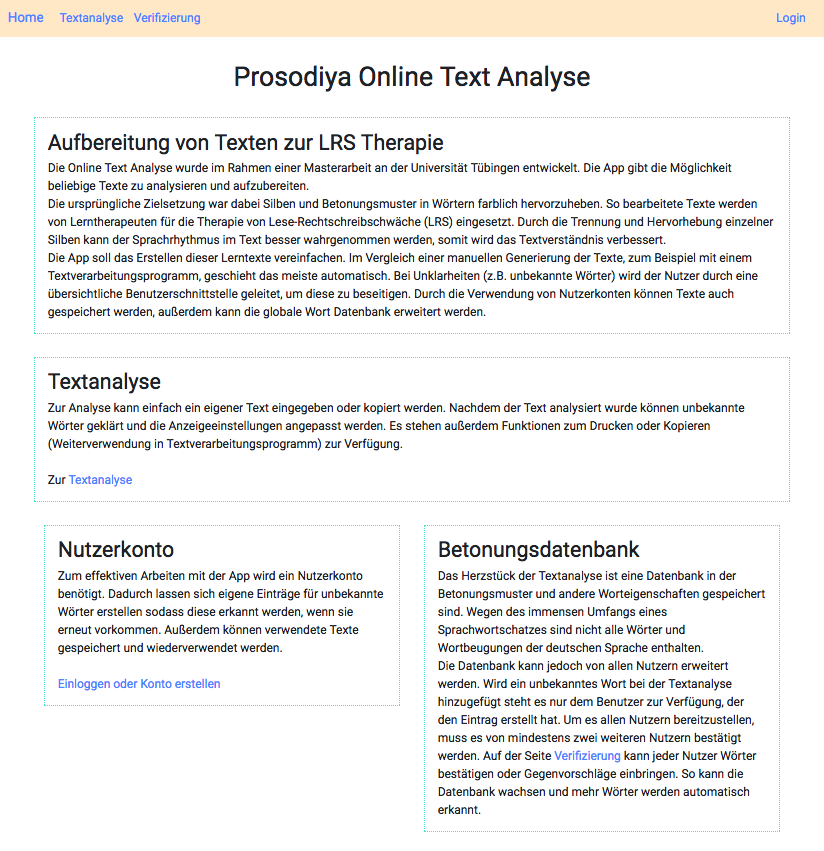
\includegraphics[width=.6\linewidth, frame]{figures/frontend/home}
	\caption{Bildschirmfoto der Begrüßungsseite}
	\label{fig:frontend-home}
\end{figure}

Die Begrüßungsseite (Abbildung \ref{fig:frontend-home}) \textit{home\_component} beinhaltet keine Programmlogik. Sie ist der Einstiegspunkt der Web-Applikation und stellt eine Übersicht über die gebotenen Funktionen dar. In den oberen zwei Kästen findet die Nutzerin oder der Nutzer eine kurze Einführung in die Software und ihre Anwendung, sowie eine Erklärung der Textanalyse Funktion. Darunter befinden sich nebeneinander zwei Kästen, in denen die Nutzerkontoverwaltung und der Verifizierungsprozess für die Wortdatenbank erklärt werden.

\subsection{Datenmodell}

Im Folgenden wird ein Überblick über das Datenmodell gegeben, dessen Klassen diverse Komponenten der Applikation benutzen. Die Klasse \texttt{AnnotationText} wird instantiiert wenn ein neuer Text analysiert wird. Sie
enthält eine Liste von Wörtern (Klasse \texttt{Word}), welche wiederum eine Liste von Silben (Klasse \texttt{Syllable}) speichern. \\

\todo{Klassendiagramm AnnotationText, Word, Syllable}

Diese Klassen enthalten auch Informationen zu HTML Klassen und CSS Styles. Durch entsprechende Zugriffe können diese dann direkt im Angular HTML Template ausgelesen werden. Mit dieser Vorgehensweise ist es möglich, die Textvorschau direkt und verzögerungsfrei nach einer Nutzereingabe anzupassen. Wird zum Beispiel eine Silbenfarbe geändert wird erst über alle Wörter und Silben im \texttt{AnnotationText} iteriert und die entsprechenden CSS Farben (z.B. \texttt{color} oder \texttt{background-color}) auf die neue Farbe gesetzt. Der Angular Update Cycle \todo{heisst das so?} detektiert die Veränderung im Modell und passt das Document Object Model (DOM) der Webseite automatisch an. Es musste kein manueller Code geschrieben, durch \textit{Data Binding} werden die aktuellen Werte im Modell (Dart Klassen) sofort automatisch in das DOM übernommen.\\

Zur Verwaltung von Vorlagen zur Einstellung der Annotation wird die Klasse \texttt{TextConfiguration} verwendet. Sie enthält alle Einstellungen, die auf einen Text angewandt werden können, z.B. die Farben von betonter und unbetonter Silben, Silben- und Wortabstände oder das Silbentrennzeichen. Außerdem beinhaltet sie eine Instanz der Klasse \texttt{PartOfSpeech}, welche spezielle Annotationseinstellungen für die verschiedenen Wortarten speichert.
\todo{Klassendiagramm TextConfiguration und PartOfSpeech}\\

Die Klasse \texttt{UserEntry} bildet die manuell segmentierten Wörter ab, die dem System unbekannt waren und vom Nutzer selbst erstellt wurden. Ein \texttt{UserEntry} enthält Informationen über Worttext, Wortart, Segmentierung der Silben und Wortbetonung. Vom Nutzer angelegte, eigene Texte werden in der Klasse \texttt{UserText} (mit dem Wortlaut des Texts und einem Titel) abgebildet.
\todo{Klassendiagramm von UserEntry und UserText}

\subsection{Textanalyse}

Die Text Analyse stellt das Herzstück der Applikation dar und ist in der Komponente \textit{text\_analysis\_component} abgebildet. Sie bindet mehrere Subkomponenten ein, die in den folgenden Abschnitten vorgestellt werden. Es gibt Nutzeroberflächen für
\begin{itemize}
	\item die Eingabe neuer Texte,
	\item die Vorschau des aktuell analysierten Texts,
	\item sowie die Manuelle Analyse dem System unbekannter Wörter.
\end{itemize}

\begin{figure}[h!]
	\centering
	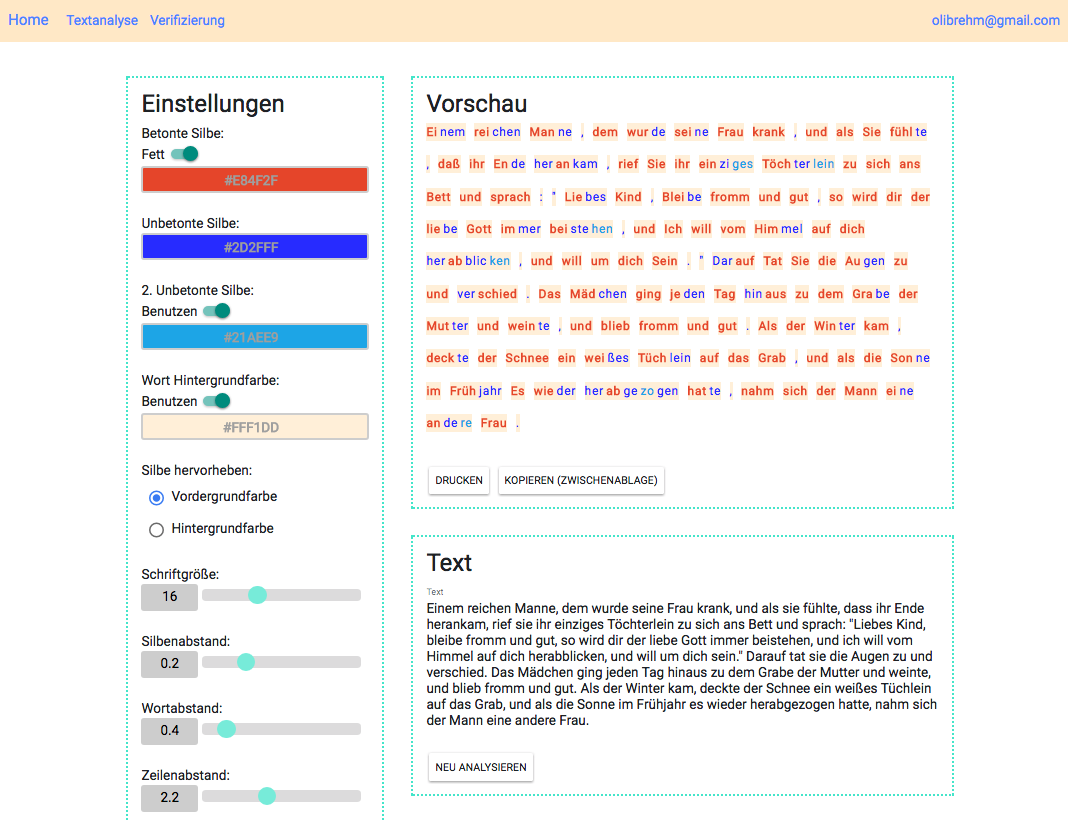
\includegraphics[width=.8\linewidth, frame]{figures/frontend/textanalyse}
	\caption{Bildschirmfoto der Textanalyse}
	\label{fig:frontend-textanalyse}
\end{figure}

\subsubsection{Texteingabe}

Ist noch kein Text analysiert, so zeigt die Text Analyse ein leeres Eingabetextfeld (in Komponente \textit{text\_analysis\_component}). Hier kann ein beliebiger Text eingetippt und analysiert werden.

\begin{figure}[h!]
	\centering
	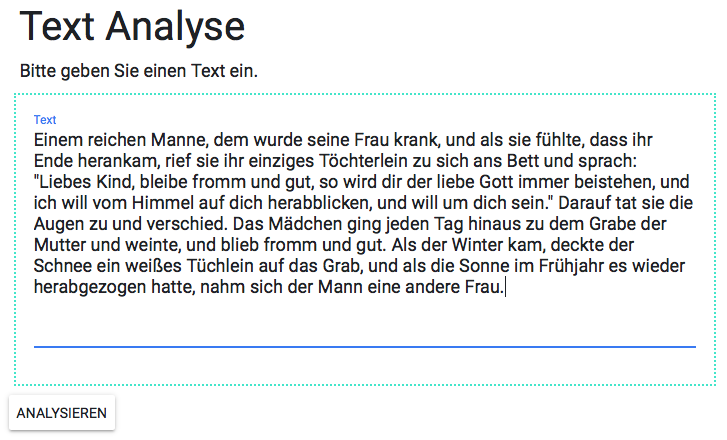
\includegraphics[width=.6\linewidth, frame]{figures/frontend/texteingabe}
	\caption{Bildschirmfoto der Texteingabe}
	\label{fig:frontend-texteingabe}
\end{figure}

\subsubsection{TextAnalysisService}

Der \texttt{TextAnalysisService} wird von mehreren Komponenten verwendet und verwaltet vor Allem eine Instanz der Klasse \texttt{AnnotationText}. Er beinhaltet auch die Logik um einen Eingabetext zu analysieren. Dazu wird ein HTTP Request mit dem Eingabetext an das Backend geschickt. Aus der Antwort kann das Modell des annotierten Texts aufgebaut und in der Vorschau angezeigt werden. Der Service bietet zudem die Funktionen zum Anwenden der aktuellen Annotationseinstellung auf den Text.

\subsubsection{Textvorschau}

Die Textvorschau (Komponente \textit{text\_preview\_component}, gezeigt in Abbildung \ref{fig:frontend-textanalyse}) stellt das Ergebnis der Textannotation so dar, wie es auch im Druck aussehen würde. Die Informationen über die Darstellung (HTML Klassen, CSS Attribute) sind jeweils schon im Datenmodell (in den Wörtern und Silben des \texttt{AnnotationText}) gespeichert und werden im Template der Komponente nur abgerufen. Im Template wird mithilfe von Angular Direktiven über alle Wörter und Silben des Texts iteriert, je nach Typ des Wortes werden verschiedene HTML Tags eingesetzt:
\begin{itemize}
	\item Für jedes annotierte Wort und jede Silbe wird ein \texttt{span} erstellt. Die Klassen und CSS Attribute der  Spans werden mit \textit{Data Binding} (\texttt{[ngClass]} und \texttt{[ngStyle]}, s. Abschnitt \ref{sec:angulardart}) dem Modell entnommen.
	
	\item Für im Text vorkommende Linebreaks (diese werden als \texttt{Word} mit speziellem Typ dargestellt) wird jeweils ein \texttt{<br>} Tag eingesetzt.
	
	\item Für Wörter, welche bei der Analyse nicht in der Datenbank gefunden wurden, wird ein Link (\texttt{span} mit \texttt{(click)} Event) eingesetzt, welcher zur manuellen Wortanalyse (Abschnitt \ref{sec:manuelleanalyse}) führt.
\end{itemize}

Jedes annotierte Wort enthält außerdem eine Subkomponente \texttt{word\_detail\_component}, die beim Klicken auf das Wort als Popup sichtbar gemacht wird. Dieses Popup (Abbildung \ref{fig:frontend-wordconf}) enthält folgende Einstellungen, die für jedes Wort manuell angepasst werden können (eine Änderung hier verändert die grundlegenden Texteinstellungen nicht und hat auch keine Auswirkungen auf die Wortdatenbank oder manuelle Nutzereinträge).

\begin{itemize}
	\item Wort annotieren oder nicht (wird diese Option ausgeschaltet, so wird das Wort ohne Silbentrennung und in der Farbe der unbetonten Silben dargestellt)
	\item Manuelles Betonungsmuster (gilt nur für dieses Wort)
	\item Manuelle Silbentrennung (gilt nur für dieses Wort)
	\item Gleiche Wörter übernehmen (beim Klicken dieses Buttons werden in der Vorschau alle Wörter mit dem gleichen Text genauso annotiert, das ist z.B. bei häufig vorkommenden Eigennamen sinnvoll)
	\item Wortart und Lemma (diese werden nur angezeigt und können nicht verändert werden)
\end{itemize}

\begin{figure}[h!]
	\centering
	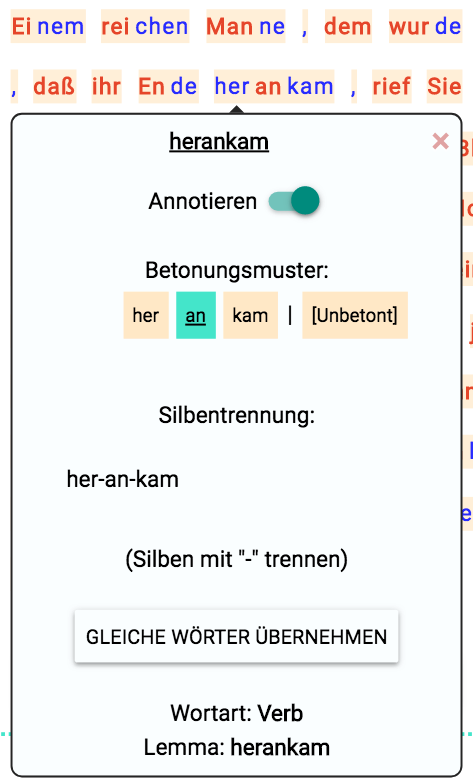
\includegraphics[width=.4\linewidth, frame]{figures/frontend/wordpopup}
	\caption{Bildschirmfoto der spezifischen Worteinstellungen}
	\label{fig:frontend-wordconf}
\end{figure}

Zusätzlich sind im Vorschaufenster Buttons für das Drucken und Kopieren des Texts vorhanden.
\begin{itemize}
	\item Der \textit{Drucken} Button öffnet den Drucken Dialog des verwendeten Browsers. Damit nur der Text in der Vorschau gedruckt wird, wird hier ein eigener CSS Style verwendet. Mit der \texttt{@media print} CSS Anweisung werden dafür alle nicht im Druck benötigten HTML Tags auf \texttt{display: none} gesetzt. und somit ausgeblendet. Zudem wird die Größe des Textvorschau Tags verändert. Ist auf dem Nutzersystem ein PDF Drucker installiert, kann der Text so auch als PDF gespeichert werden.
	
	\item Der Button \textit{Kopieren (Zwischenablage)} kopiert automatisch nur den Vorschautext samt Annotation in die Zwischenablage, sodass dieser z.B. in einem externen Textverarbeitungsprogramm weiter bearbeitet werden kann.
\end{itemize}

\subsubsection{Manuelle Wortanalyse}
\label{sec:manuelleanalyse}

Ist bei der Analyse dem System ein Wort nicht bekannt, so wird es in der Textvorschau rot hinterlegt. Beim Klicken auf das Wort öffnet sich die Manuelle Wortanalyse (Komponente \textit{word\_review\_component}), in der der die Nutzerin oder der Nutzer für dieses Wort das Betonungsmuster und die Silbentrennung selbst bestimmen kann. Hierfür gibt es zum Einen ein Auswahlfenster für die betonte Silbe (durch Klicken kann diese bestimmt werden und wird bei Auswahl in deiner anderen Farbe dargestellt) und zum Anderen ein Textfeld für die Silbentrennung. Hier können manuell Trennstriche gesetzt werden, wobei der Text des Wortes selbst nicht verändert werden darf. Ändert sich bei entsprechender Eingabe die Silbentrennung, passt sich die Eingabe für das Betonungsmuster automatisch an. Mit entsprechenden Buttons kann die Nutzerin oder der Nutzer dann die vorgenommene Analyse entweder speichern, das Wort im Text ignorieren oder ohne zu speichern zum Text zurückkehren.\\

Um die manuellen Eingaben zu erleichtern und zu minimieren werden außerdem automatische Vorschläge generiert. Das Backend sendet für jedes zu bearbeitende Wort eine Liste von Vorschlägen, die aus verschiedenen Quellen stammen können (s. Abschnitt \ref{sec:segmentation-proposals}). Durch Anklicken eines Vorschlags wird dieser in den Eingabefenstern auf der linken Seite übernommen.

\todo{irgendwo muss noch segmentation service und segmentation proposal service rein}

\begin{figure}[h!]
	\centering
	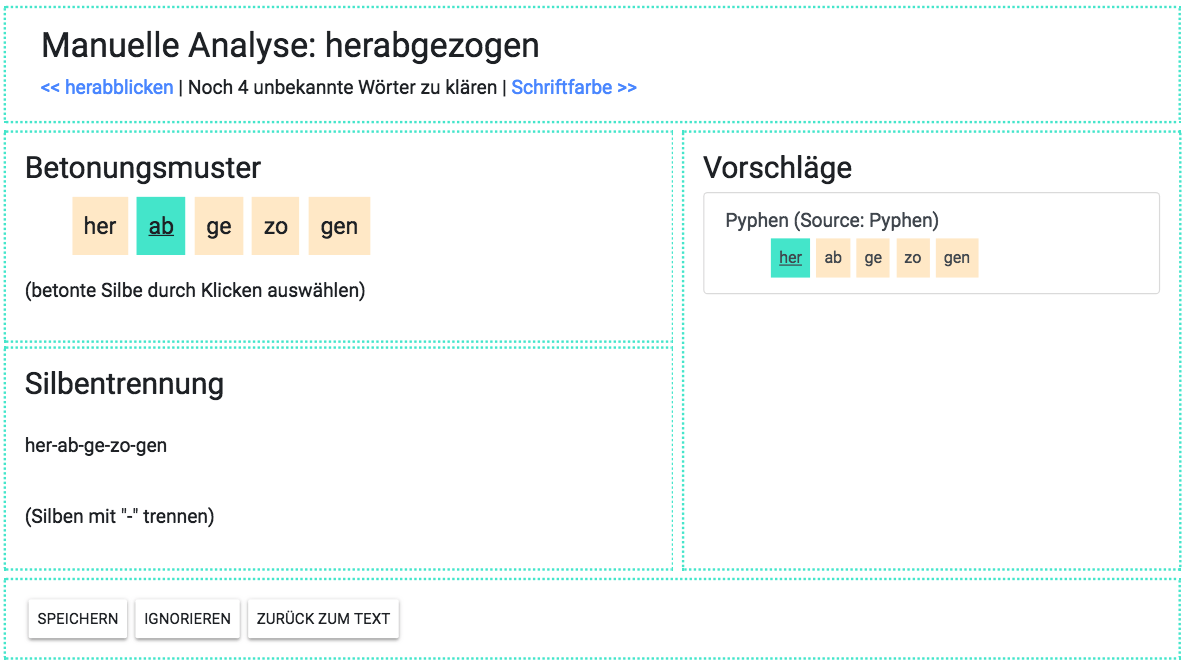
\includegraphics[width=.8\linewidth]{figures/frontend/manuelle-analyse}
	\caption{Bildschirmfoto der Manuellen Wortanalyse\todo{bild wo MARY funktioniert!}}
	\label{fig:frontend-manuelle-analyse}
\end{figure}

\subsubsection{Textoptionen}

Unter dem Textvorschaufenster befinden sich weitere Fenster zur Verwaltung des aktuellen Texts (Komponente \texttt{text\_input\_component}). Folgende Funktionen (in drei Kästen, von oben nach unten) werden hier noch angeboten:
\begin{itemize}
	\item Der aktuelle Text wird in einem Eingabefeld angezeigt. Dieser kann hier verändert und neu analysiert werden.
	\item Der aktuelle Text kann im Nutzerkonto (s. Abschnitt \ref{sec:nutzerkonto}) gespeichert werden. Dazu muss ein Titel eingegeben werden. Wird anschließend der \textit{Speichern} Button gedrückt, wird der Text mit zugehörigem Titel vom \texttt{UserAccountService} gespeichert.
	\item Die aktuelle Analyse kann vollständig verworfen werden, sodass wieder das ursprüngliche, leere Textfeld angezeigt wird.
\end{itemize}

\subsection{Annotationseinstellungen}

Im Kasten links neben der Textvorschau können die Einstellungen verändert werden, die die Art der Annotation bestimmen. Die Einstellungen werden zentral in einem Objekt der Klasse \texttt{TextConfiguration} im \texttt{TextAnalysisService} gespeichert und nach Nutzereingaben auf den aktuellen Text angewandt. Wird hier eine Farbe oder ein Abstand verändert, so ist dies sofort in der Textvorschau sichtbar. Außerdem kann die aktuelle Konfiguration jederzeit als Vorlage gespeichert werden, so kann sie später (z.B. für einen anderen Text) wiederverwendet werden. Das User Interface für die Einstellungen ist in der Komponente \texttt{text\_settings\_component} definiert.

\subsubsection{User Interfache für Einstellungen}

Ganz oben können zunächst Farben für die Annotation und die Art, wie diese verwendet werden eingestellt werden (Abbildung \ref{fig:frontend-colorconf}):

\begin{itemize}
	\item \textit{Betonte Silbe}: Hier wird die Farbe für die betonte Silbe in jedem Wort festgelegt. Außerdem kann gewählt werden, ob der Text der Silbe fett dargestellt werden soll. Für die Auswahl der Farben wurde ein entsprechend farbiger Kasten verwendet, der beim Anklicken den Farbwahldialog des Browsers öffnet.
	
	\item \textit{Unbetonte Silbe}: Alle unbetonten Silben werden in dieser Farbe dargestellt.
	
	\item \textit{2. Unbetonte Silbe}: In längeren Wörtern folgen mehrere unbetonte Silben aufeinander. Wird diese Option aktiviert, werden aufeinanderfolgende unbetonte Silben abwechselnd in den Farben der 1. und der 2. unbetonten Silbe dargestellt.
	
	\item \textit{Worthintergrundfarbe}: Ist diese Option aktiviert erhält zusätzlich jedes Wort (über Silbengrenzen hinaus) eine Hintergrundfarbe. Dies ist z.B. dann sinnvoll, wenn man große Abstände zwischen den einzelnen Silben wählt, so kann das Wort trotzdem als Einheit erfasst werden.
	
	\item \textit{Silbe hervorheben}: Hier kann gewählt werden, ob die Silbenfarben als Schriftfarbe (\textit{Vordergrundfarbe}) oder Hintergrundfarbe benutzt werden
\end{itemize}

Beispiele zu verschiedenen Einstellungen sind in der Evaluation in Abschnitt \ref{sec:annotation-results} zu finden.

\begin{figure}[h!]
	\centering
	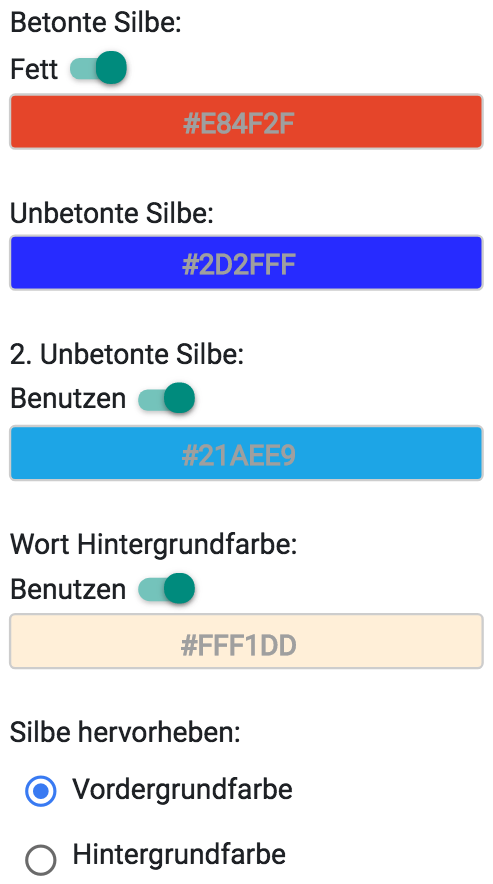
\includegraphics[width=.4\linewidth, frame]{figures/frontend/config-color}
	\caption{Bildschirmfoto der Farbeinstellungen}
	\label{fig:frontend-colorconf}
\end{figure}

Unter den Farbeinstellungen lassen sich verschiedene Größen und Abstände im Text definieren (Abbildung \ref{fig:frontend-textconf}):
\begin{itemize}
	\item Schriftgröße
	\item Silbenabstand (Abstand zwischen einzelnen Silben)
	\item Wortabstand (Abstand zwischen ganzen Wörtern)
	\item Zeilenabstand
	\item Zeichenabstand (Abstand zwischen den einzelnen Buchstaben eines Wortes)
\end{itemize}

\begin{figure}[h!]
	\centering
	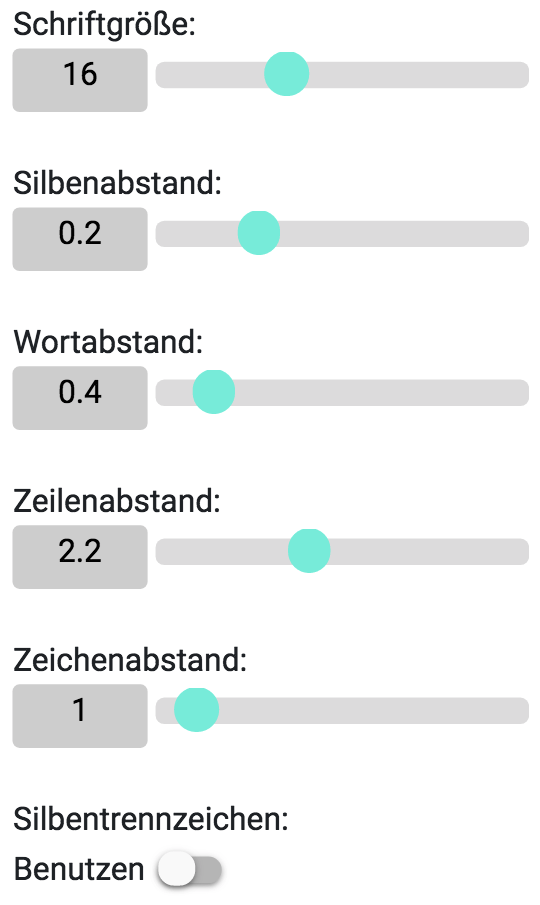
\includegraphics[width=.4\linewidth, frame]{figures/frontend/config-text}
	\caption{Bildschirmfoto der Texteinstellungen}
	\label{fig:frontend-textconf}
\end{figure}

Alle Werte lassen sich hier mithilfe eines Sliders einstellen. Außerdem gibt es die Möglichkeit, ein beliebiges Zeichen als Silbentrennzeichen zu benutzen, was dann im Zwischenraum zwischen allen Silben im Text erscheint.\\

An letzter Stelle in den Einstellungen steht ein Dropdown Menü, in dem man eine Wortart auswählen kann (Abbildung \ref{fig:frontend-pos-einstellungen}). Für jede Wortart lassen sich folgende Einstellungen vornehmen, die dann auf den gesamten Text angewandt werden:
\begin{itemize}
	\item \textbf{Annotieren}: Aktiviert die Annotation für Wörter dieser Wortart, d.h. Silben werden getrennt und in den gewählten Farben dargestellt).
	
	\item \textbf{Unbetont}: Die Annotation ist zwar aktiv und Silben werden getrennt dargestellt, allerdings wird die betonte Silbe nicht besonders hervorgehoben.
	
	\item \textbf{Ignorieren}: Das Wort wird ohne Trennung von Silben in der Farbe der unbetonten Silbe dargestellt.
\end{itemize}

Ändert die Nutzerin oder der Nutzer eine Einstellung, so wird im \texttt{AnnotationText} über sämtliche Wörter iteriert und deren Einstellung entsprechend angepasst.

\begin{figure}[h!]
	\centering
	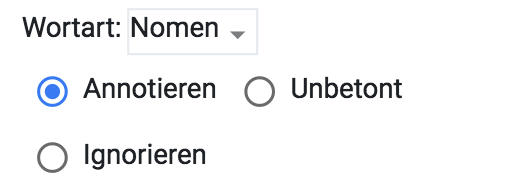
\includegraphics[width=.4\linewidth, frame]{figures/frontend/config-pos}
	\caption{Bildschirmfoto der spezifischen Wortart Einstellungen}
	\label{fig:frontend-pos-einstellungen}
\end{figure}

\subsubsection{Annotationsvorlagen}

Im Kasten unterhalb der Annotationseinstellungen können Konfigurationen verwaltet werden. Jedem Nutzerkonto sind Vorlagen zugeordnet, d.h. jede Nutzerin und jeder Nutzer verwaltet und sieht nur ihre oder seine eigenen Vorlagen. In der Vorlage werden sämtliche Einstellungen gespeichert, das ganze \texttt{TextConfiguration} Objekt wird hier an das Backend geschickt und serialisiert.\\

Sind bereits Vorlagen vorhanden, werden diese hier aufgelistet. Sie können ausgewählt (und damit auf den aktuellen Text angewandt) werden oder durch Klicken auf das kleine \textit{X} rechts neben dem Vorlagennamen gelöscht werden. Darunter befindet sich ein Textfeld für den Namen einer neu anzulegenden Vorlagen. Beim Klicken des \textit{Vorlage speichern} Buttons wird diese dann unter dem gewählten Namen (und mit den momentan aktiven Einstellungen) neu gespeichert oder, wenn die Vorlage schon existiert überschrieben.

\begin{figure}[h!]
	\centering
	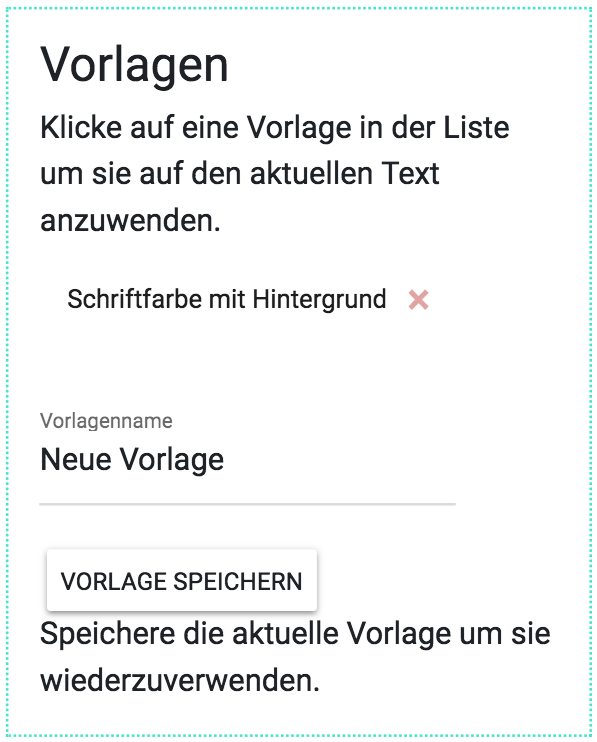
\includegraphics[width=.4\linewidth]{figures/frontend/config-vorlagen}
	\caption{Bildschirmfoto der UI zur Verwaltung und Verwendung von Annotationsvorlagen}
	\label{fig:frontend-vorlagen}
\end{figure}

\subsection{Nutzerkonto}
\label{sec:nutzerkonto}

Die Nutzerkonto Seite zeigt entweder das Formular zum Einloggen oder Konto erstellen an, oder falls die Nutzerin oder der Nutzer schon eingeloggt ist, Informationen und Inhalte des Nutzerkontos. Die Komponente \texttt{user\_account\_component} lagert einige Funktionalitäten wie die Registrierung oder die Liste von Nutzertexten in Subkomponenten aus.

\subsubsection{UserAccountService}

Der \texttt{UserAccountService} speichert die Informationen zum aktiven Nutzerkonto, z.B. Email Adresse und Passwort, sowie eine Liste von Nutzertexten und manuell segmentierten Wörtern. Er bildet alle Funktionen ab (z.B. Anglegen, Auflisten oder Löschen), die zum Verwalten von Nutzerkonten, Nutzertexten und Wörtern notwendig sind. Dafür werden jeweils HTTP Requests an das Backend gesendet und die erhaltenen Antworten weiter verarbeitet.

\subsubsection{Login und Registrierung}

Ist kein Nutzer eingeloggt, so wird zuerst das Login Formular angezeigt. Außerdem lautet der Link rechts oben in der Navigationsleiste \textit{Login}, sodass der Login schnell gefunden werden kann. Loggt sich eine Nutzerin oder ein Nutzer mit einem bereits bestehenden Konto ein, so enthält der Navigationslink die Email Adresse des Nutzerkontos.\\

Unter dem Login Formular führt ein Link mit der Aufschrift \textit{Neues Konto erstellen} auf die Registrierungsseite. Hier muss für die erfolgreiche Registrierung eine Email Adresse sowie ein Passwort eingegeben werden. Außerdem speichert das Nutzerkonto Vor- und Nachname, sowie die Information, ob es sich bei dem neu anzulegenden Konto um ein Expertenkonto handelt, was in einer Checkbox angegeben werden kann. Expertenkontos sollen von SprachtherapeutInnen oder NachhilfelehrerInnen genutzt werden.  Diese verfügen bei der Verifizierung über eine schwerer gewichtete Stimmt (s. Abschnitt \ref{sec:verification-service}). Wird die Registrierung abgeschickt wird das neue Nutzerkonto im Backend erstellt und die Nutzerkontoseite kehrt zum Login Formular zurück. Schlägt das Registrieren fehl (z.B wenn es schon ein Konto mit der eingegebenen Email Adresse gibt, oder weil Eingaben fehlen) wird eine entsprechende Fehlermeldung angezeigt.

\subsubsection{Nutzerkonto Seite}

Ist aktuell eine Nutzerin oder ein Nutzer eingeloggt, werden Informationen zum Konto, sowie Listen von gespeicherten Texten und manuell segmentierten Wörtern angezeigt.\\

Die Liste der gespeicherten Nutzertexte zeigt zunächst nur deren Titel als Links an (Komponente \texttt{user\_textlist\_component}). Werden diese angeklickt, sieht man den Text und hat die Möglichkeit, diesen für die Analyse zu verwenden oder zu löschen. Klickt man auf den Button \textit{Verwenden}, wechselt die Applikation zur Textanalyse und analysiert den gewählten Text. \\

Unter der Textliste ist die Liste manuell segmentierter Wörter zu finden (Komponente \texttt{user\_wordlist\_component}). Die Einträge zeigen den Worttext, die Silbentrennung und das Betonungsmuster der Segmentierung. Die Einträge können auch gelöscht werden, z.B. falls ein Fehler bei deren Erstellung unterlaufen ist.\\

Ganz unten auf der Seite sind Buttons zum Ausloggen und Löschen des Kontos vorhanden.

\begin{figure}[h!]
	\centering
	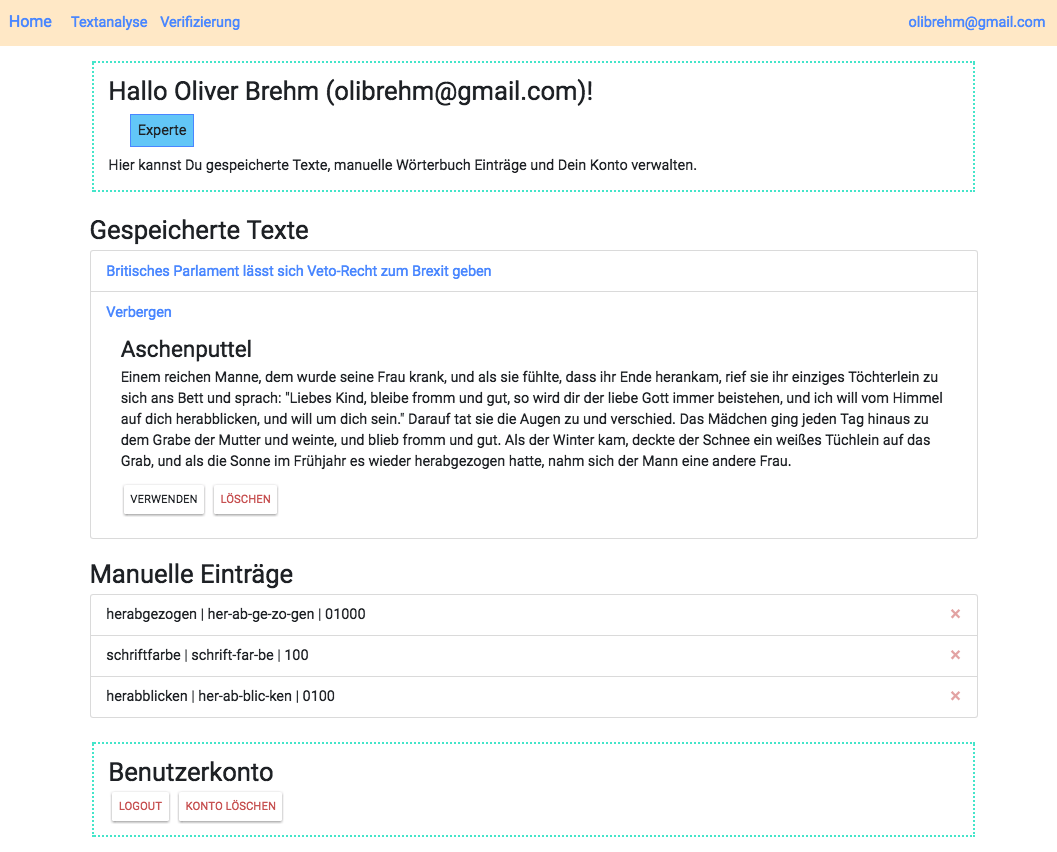
\includegraphics[width=.8\linewidth, frame]{figures/frontend/user-account}
	\caption{Bildschirmfoto der Nutzerkontoseite}
	\label{fig:frontend-useraccount}
\end{figure}

\subsection{Wort-Verifizierung}

Die Wort Verifizierung dient der Bestätigung von manuellen Segmentierung von NutzerInnen durch andere NutzerInnen, sodass diese in die globale Wortdatenbank aufgenommen werden können (s. Abschnitt \ref{sec:verification-service}). Das User Interface für diesen Prozess ist in der Komponente \texttt{word\_verification\_component} implementiert.\\

Ist eine Nutzerin oder ein Nutzer eingeloggt, werden nacheinander zu verifizierende Wörter geladen, das User Interface ähnelt dem, das zur manuellen Analyse von unbekannten Wörtern verwendet wird (s. Abschnitt \ref{sec:manuelleanalyse}). Auch hier gibt es jeweils eine Eingabemöglichkeit zur Auswahl der betonten Silbe und zur Bestimmung der Silbentrennung. Auf der Rechten Seite befinden sich allerdings neben den automatisch generierten Vorschlägen auch die Segmentierungsvorschläge anderer NutzerInnen. Automatisch wird der Vorschlag der Nutzerin oder des Nutzers ausgewählt, die die Segmentierung zuerst erstellt hat. Haben weitere NutzerInnen den Vorschlag schon verifiziert, so erscheinen auch deren Segmentierungen in der Liste. \\

Zur eigentlichen Verifizierung kann nun ein Eintrag in der Liste der Vorschläge ausgewählt werden oder, falls alle Vorschläge als falsch empfunden werden, ein andere Segmentierung auf der linken Seite eingestellt werden. Danach wird die Verifizierung mit dem Button \textit{Abschicken} gespeichert.\\
Sind noch weitere zu verifizierende Einträge vorhanden, wird sofort das nächste Wort geladen. Ein Label unter der Überschrift der Komponente zeigt an, wie viele zu verifizierende Wörter es noch gibt.

\begin{figure}[h!]
	\centering
	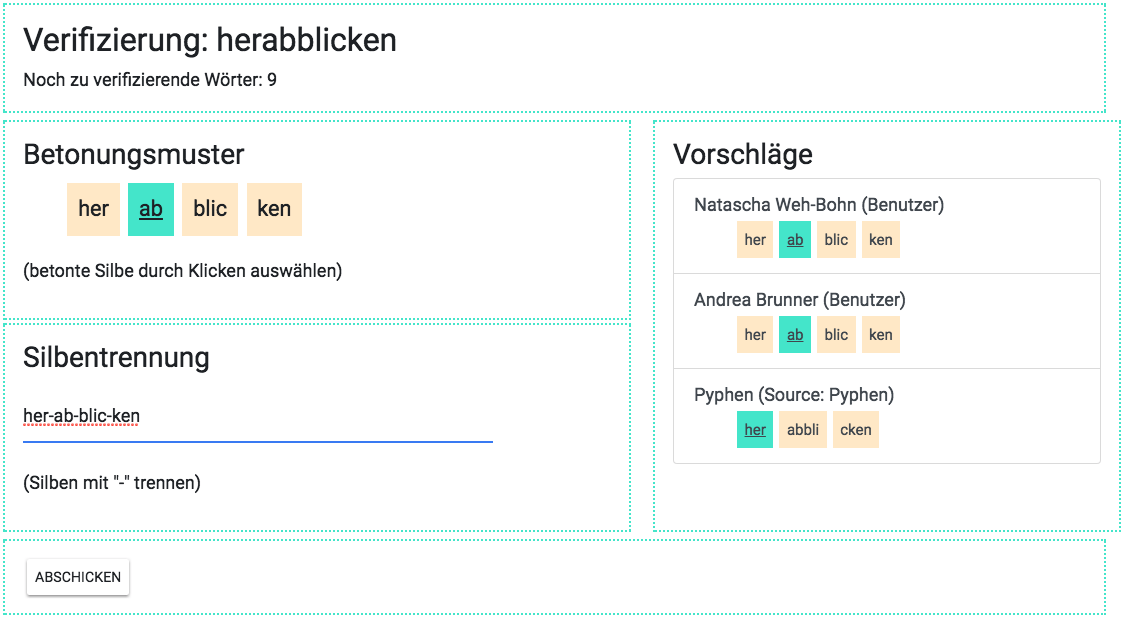
\includegraphics[width=.8\linewidth]{figures/frontend/verifizierung}
	\caption{Bildschirmfoto der Verifikation von manuell hinzugefügten Wörtern}
	\label{fig:frontend-verification}
\end{figure}
\cleardoublepage

% !TEX root = ../ausarbeitung.tex

\chapter{Evaluation}

Die Applikation wurde mit dem Hauptziel entwickelt, eine Nutzeroberfläche zu entwickeln, mit der sowohl Personen, die in der LRS Therapie arbeiten (wie Lerntherapeuten oder Nachhilfelehrer) als auch Nicht-Experten (z.B. die Eltern betroffener Kinder) intuitiv und effizient benötigtes Arbeitsmaterial erstellen können. Außerdem wurde untersucht wie eine Datenbank für Betonungsmuster in Wörtern erstellt und benutzerfreundlich erweitert werden kann.\\

Die Evaluation untersucht daher folgende Punkte:
\begin{itemize}
	\item Erstellung von Arbeitsmaterial aus einem einfachen Text 
	\item Intuitivität und Einfachheit der Bedienung
	\item Effizienz des Prozesses der Erstellung von Arbeitsmaterial
	\item Unterschiede in der Bedienung durch Experten und Laien
	\item Nutzerfreundliche Erweiterung der Wortdatenbank
\end{itemize}

Zunächst wird durch Beispiele eines annotieren Textes mit verschiedenen Einstellungen demonstriert, welche vielseitigen Möglichkeiten die Textannotation für das Erstellen von Arbeitsmaterial bietet. Für die Untersuchung von Intuitivität, Einfachheit und Effizienz bei der Bedienung der Applikation wurde ein Nutzertest durchgeführt. Dieser fand als Interview statt um qualitative Daten durch Nutzerbefragung zu erheben. Außerdem wurden quantitative Daten durch das Ausfüllen von Ankreuzfragen während des Interview erhoben.

\section{Ergebnisse der Textannotation}

Um zu zeigen, dass die Applikation das Ziel des automatischen Erstellens von Arbeitsmaterial erfüllt, werden im Folgenden verschiedene Texte präsentiert, die mit Hilfe des Web Interfaces erstellt wurden. Die Ergebnisse zeigen, dass das Programm diese Ziel nicht nur erfüllt, sondern im Vergleich zu herkömmlichen Methoden \tocite{Silbefibel, ABC} auch noch einen hohen Grad an Flexibilität bietet. Die Einstellungen und damit das Erscheinungsbild des resultierenden Textes können vom Nutzer frei an die Bedürfnisse des jeweiligen Falls angepasst werden.\\

Im Folgenden wurde der Beispieltext \textit{Aschenputtel} mit der Web Applikation analysiert, sodass Silbentrennung und Betonung farblich markiert dargestellt werden. Die in den Beispielen verwendeten Texten wurden mit der Druckfunktion der Textvorschau als PDF Dateien exportiert. Jedes Bild entspricht einer DIN A4 Seite.

\subsubsection{Beispiel 1: Hervorhebung der Silben mit zwei alterierenden Farben}

Im ersten Beispiel wird die Schriftfarbe für da Hervorheben der Silben genutzt. Die betonte Silbe wird immer rot dargestellt, in Wörtern mit vielen Silben, werden diese dann alterierend rot und blau hervorgehoben. Die Schriftgröße wurde auf \textit{22} gesetzt, der Wortabstand auf den Wert \textit{0.4}. Zusätzlich sorgt die Einstellung des Zeilenabstands auf \textit{1.5} für bessere Lesbarkeit.

\begin{figure}[h!]
	\centering
	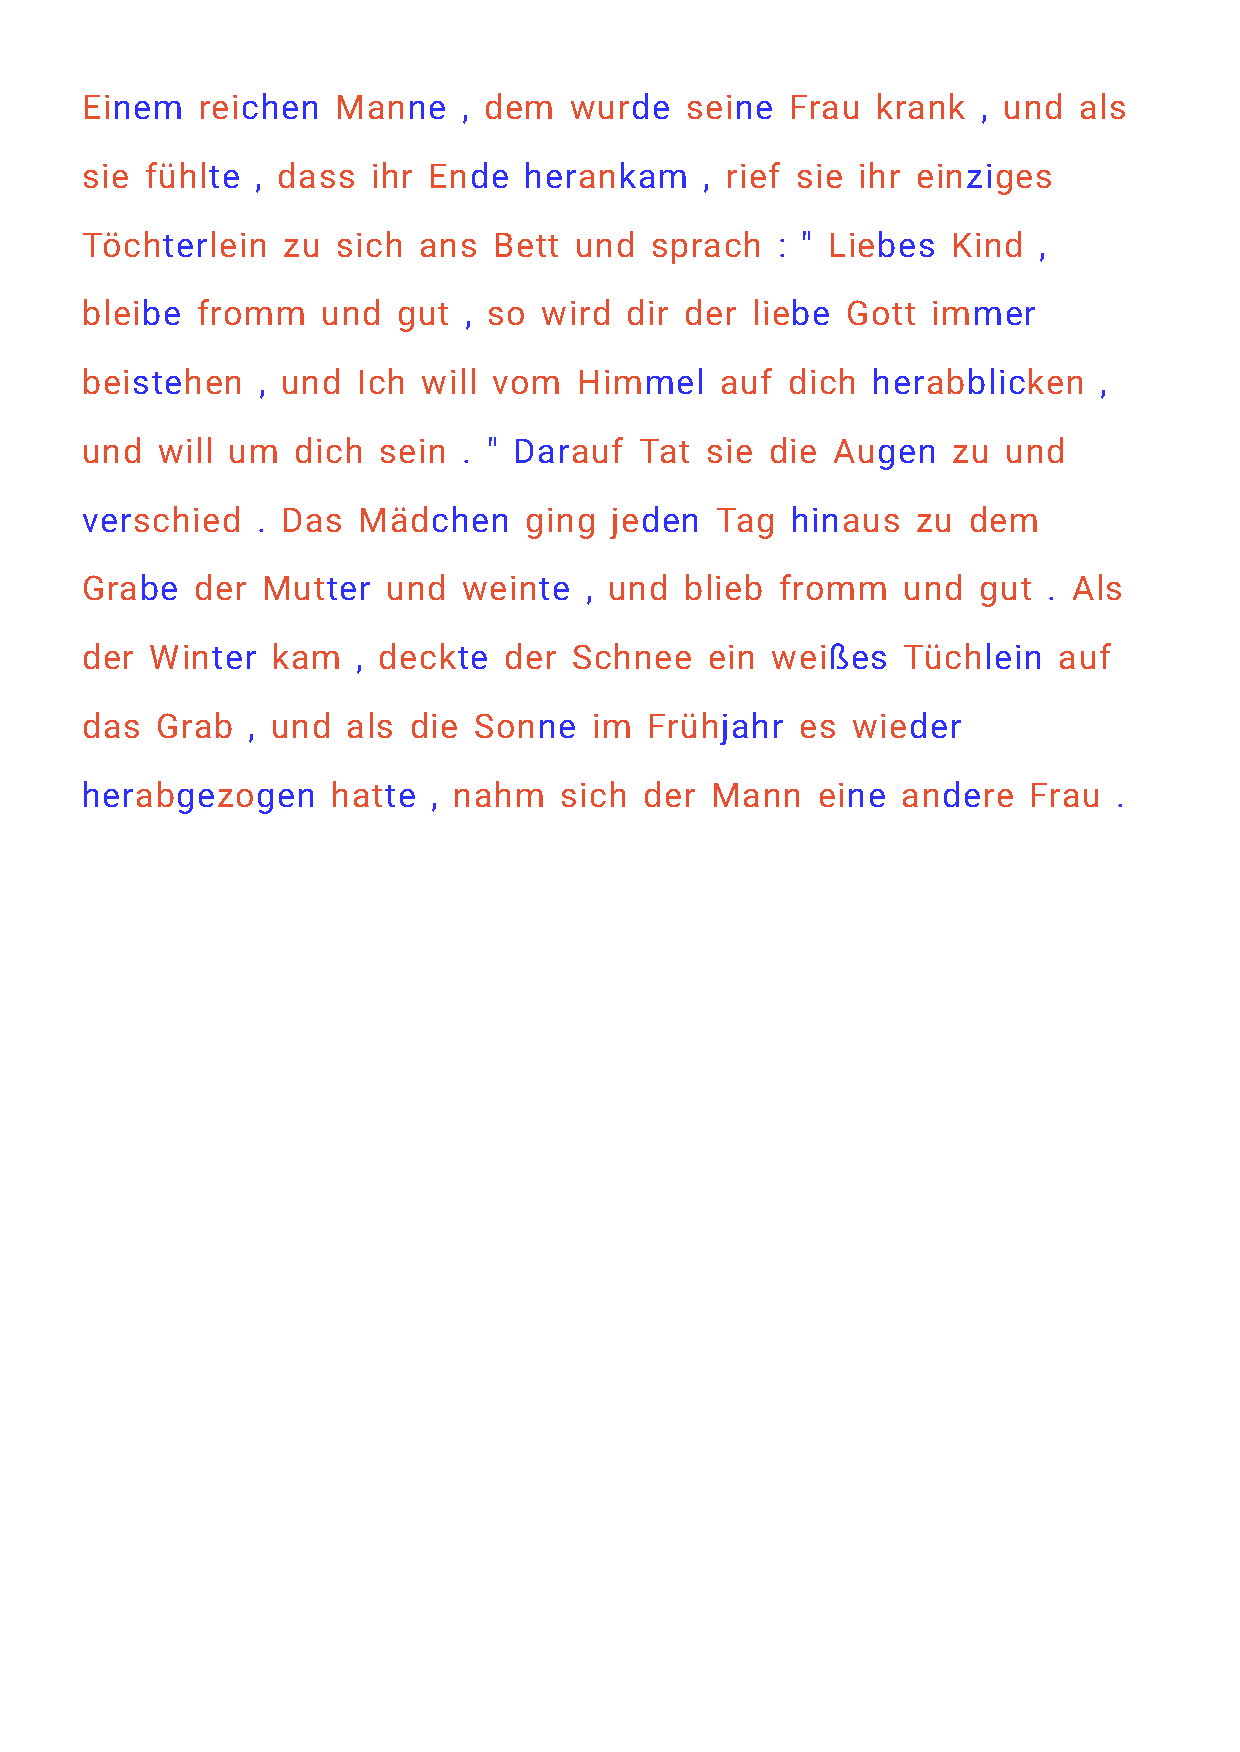
\includegraphics[width=.7\linewidth, frame]{figures/evaluation/annotation1}
	\caption{Hervorhebung der Silben mit zwei alterierenden Farben}
	\label{fig:evaluation-ex1}
\end{figure}
\newpage

\subsubsection{Beispiel 2: Worthintergrund und Silbenabstand}

In diesem Beispiel sorgt die Worthintergrundfarbe für eine bessere Wahrnehmung des Wortes als Einheit. Dadurch kann auch ein Silbenabstand (hier \textit{0.1}) eingestellt werden ohne dass die Gefahr besteht, dass dadurch nicht mehr klar ist, welche Silben zusammen gehören. Wegen dem Worthintergrund nehmen die Wörter mehr Platz in der Zeile ein, daher wurde auch der Zeilenabstand auf \textit{2.2} erhöht. Zudem wurde hier ein Zeichenabstand von \textit{2} (statt \textit{1} in Beispiel 1) gewählt.

\begin{figure}[h!]
	\centering
	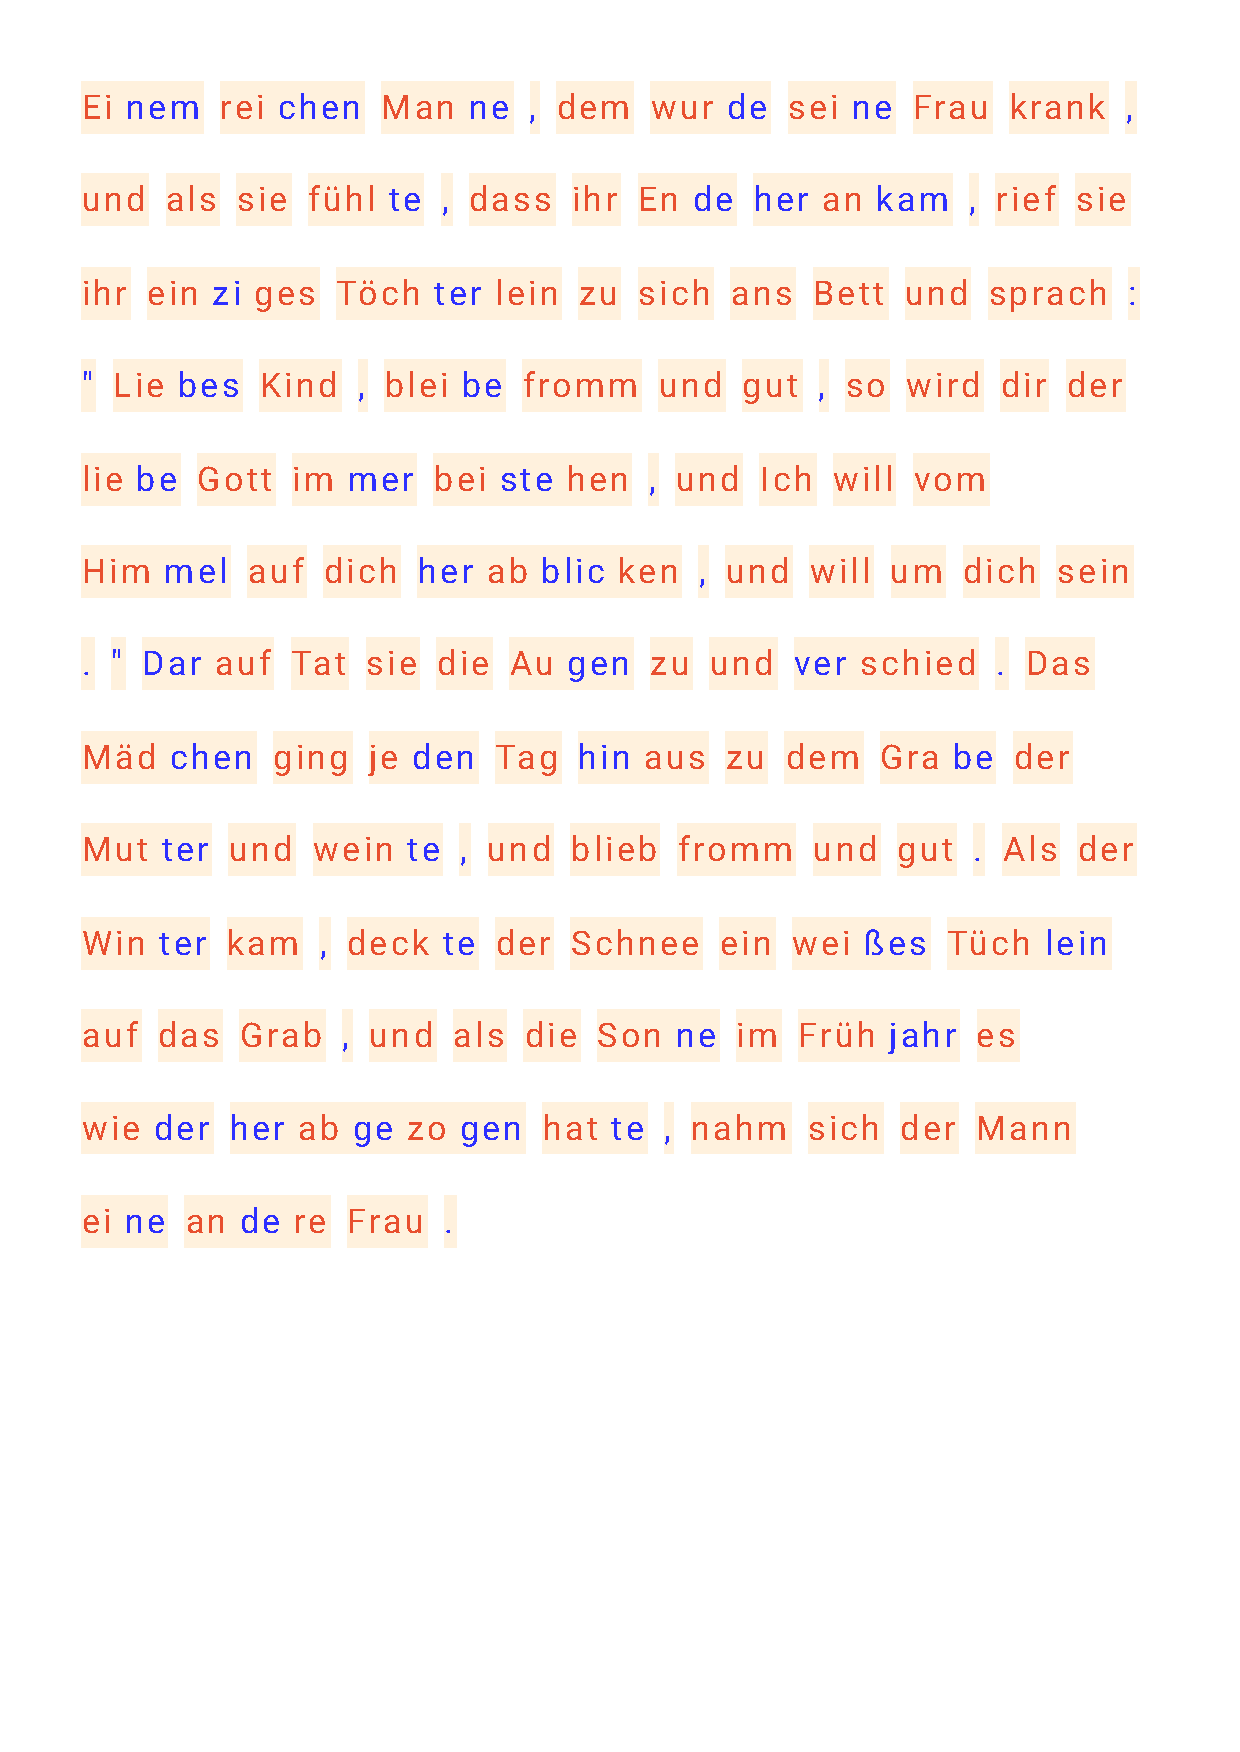
\includegraphics[width=.7\linewidth, frame]{figures/evaluation/annotation2}
	\caption{Worthintergrund und Silbenabstand}
	\label{fig:evaluation-ex2}
\end{figure}
\newpage

\subsubsection{Beispiel 3:  Silbentrennzeichen und verschiedene Silbenfarben}

In Beispiel 3 wurde wieder auf die Worthintergrundfarbe verzichtet. Das Trennzeichen \qq{=} soll hier das Silbentrennen erleichtern, sowie zusammenhängende Silben zu einem Wort gruppieren. Der Zeichenabstand beträgt wieder \textit{1}, der Silbenabstand \textit{0}, da das Gleichheitszeichen hier als Silbentrenner dient. Zusätzlich wurde eine weitere Farbe für alterierende Silben gewählt. Hier wird nur noch die betonte Silbe rot dargestellt, danach alterieren die Silben bei langen Wörtern in den Farben blau und lila.

\begin{figure}[h!]
	\centering
	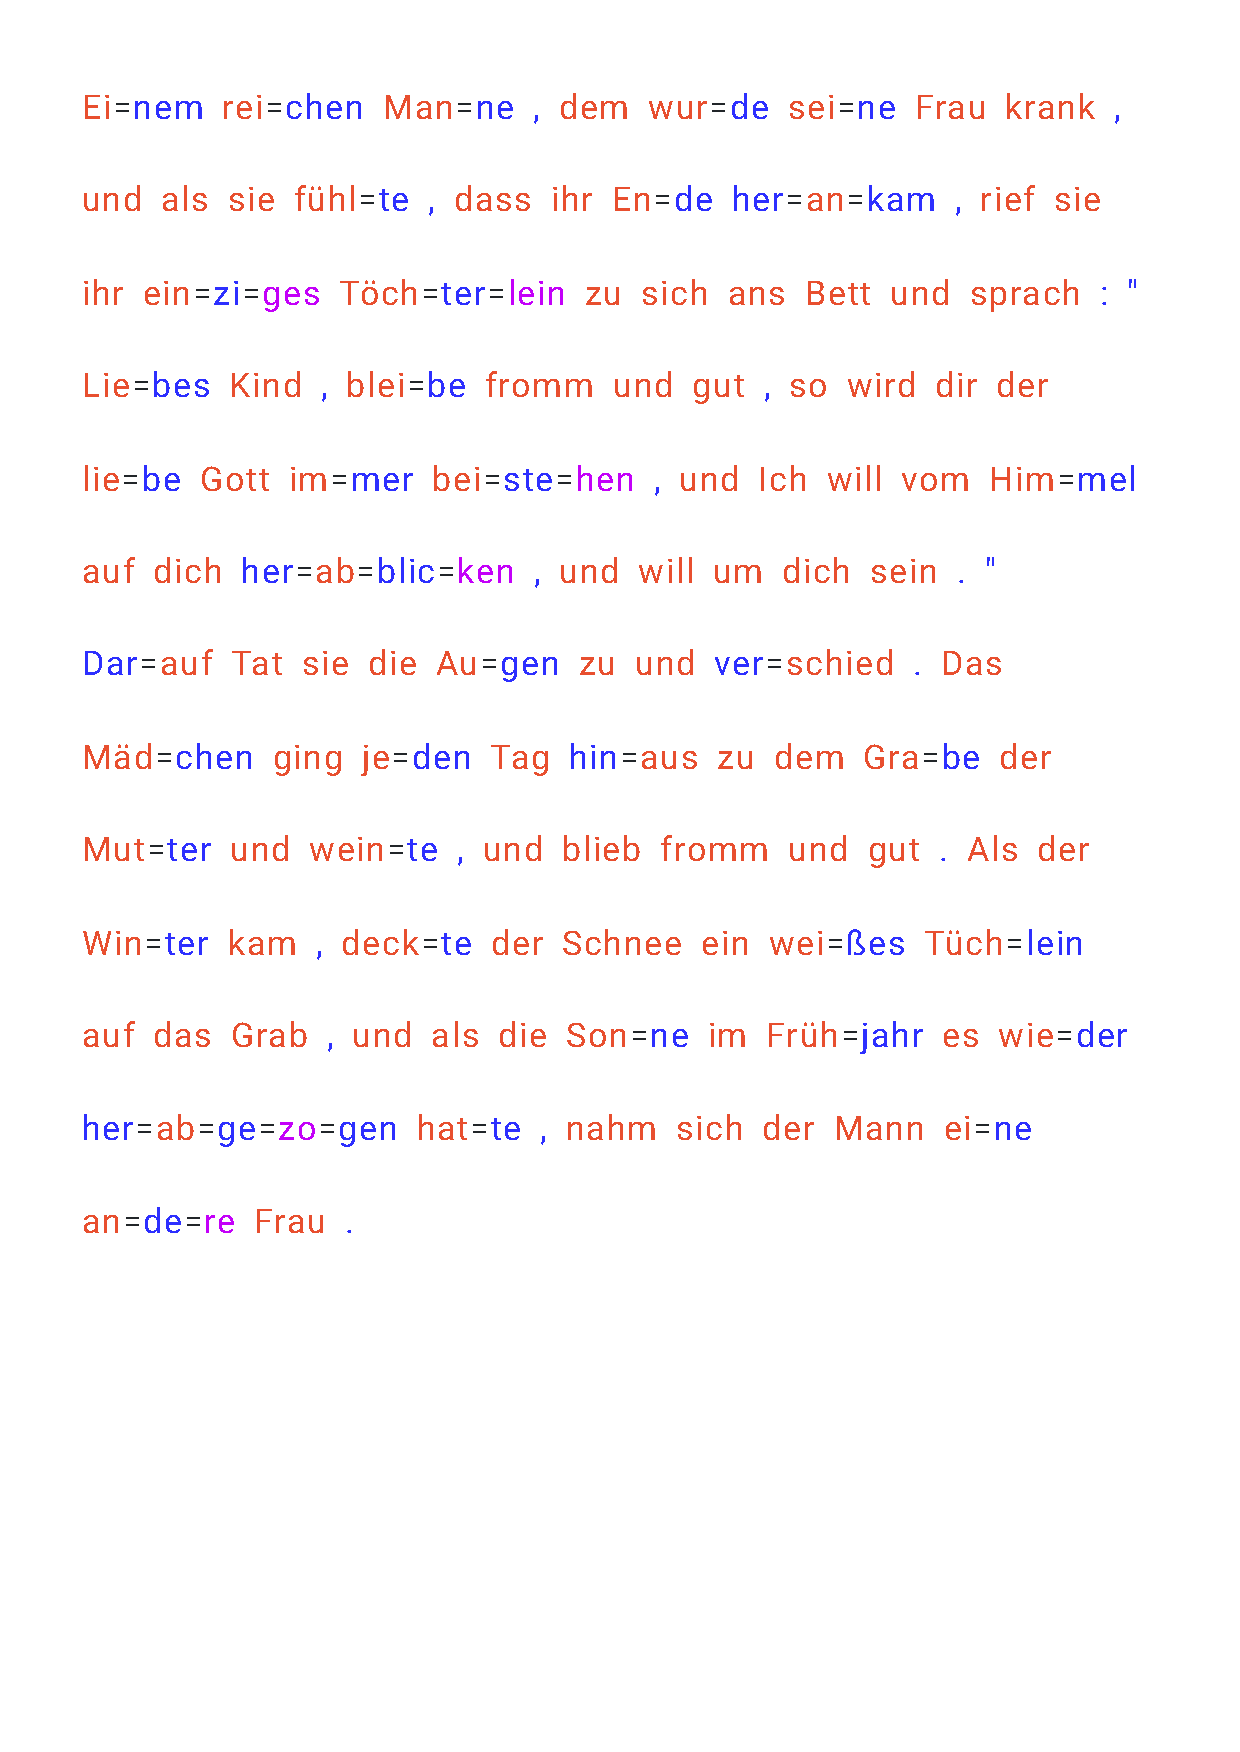
\includegraphics[width=.7\linewidth, frame]{figures/evaluation/annotation3}
	\caption{Silbentrennzeichen und verschiedene Silbenfarben}
	\label{fig:evaluation-ex3}
\end{figure}
\newpage

\subsubsection{Beispiel 4: Hervorhebung des Silbenhintergrunds}

In diesem Beispiel wird ein anderer Ansatz der farblichen Hervorhebung gewählt. Die eingestellten Farben bestimmen hier den Hintergrund der Silben und nicht die Schriftfarbe (diese ist immer Schwarz). Das Beispiel hebt vor Allem die betonte Silbe hervor, die grün dargestellt werden. Unbetonte Silben bekommen alterierend zwei verschiedene Grautöne als Hintergrund. Der Silbenabstand ist hier wieder \textit{0}, somit wird die Einheit des Wortes deutlich erkennbar.

\begin{figure}[h!]
	\centering
	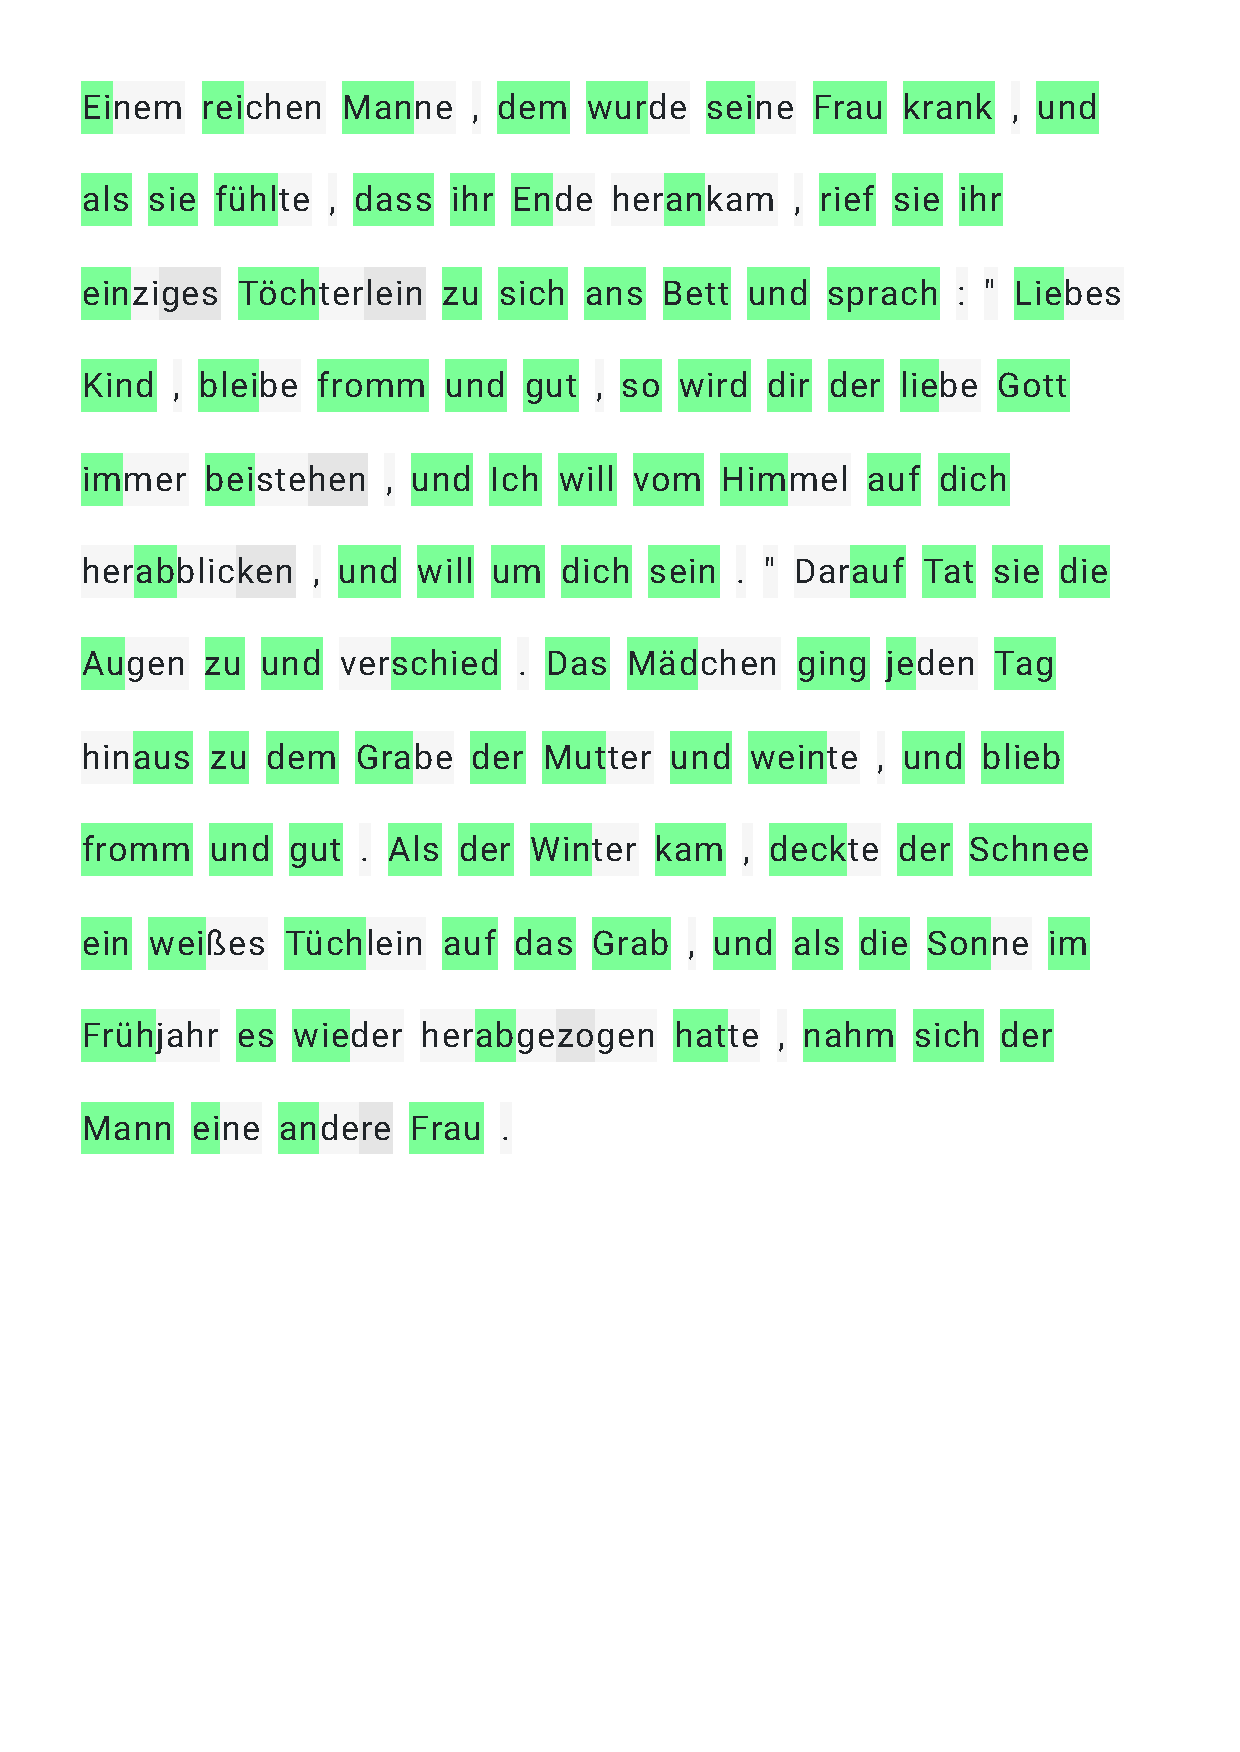
\includegraphics[width=.7\linewidth, frame]{figures/evaluation/annotation4}
	\caption{Hervorhebung des Silbenhintergrunds}
	\label{fig:evaluation-ex4}
\end{figure}
\newpage

\subsubsection{Beispiel 5: Manuelles Deaktivieren der Hervorhebung in kurzen Wörtern}

In Beispiel 5 wird der Sprachrhythmus mit Wortbetonungen noch deutlicher hervorgehoben. Die betonte Silbe wir zusätzlich zur grünen Farbe auch fett dargestellt. Außerdem wurde die Betonung in manchen Wörtern deaktiviert, so werden im ganzen Text beispielsweise Artikel, Präpositionen oder manche einsilbigen Wörter nicht betont markiert. Dieser Text soll damit einen Fokus auf den Sprachrhythmus innerhalb ganzer Sätze legen.

\begin{figure}[h!]
	\centering
	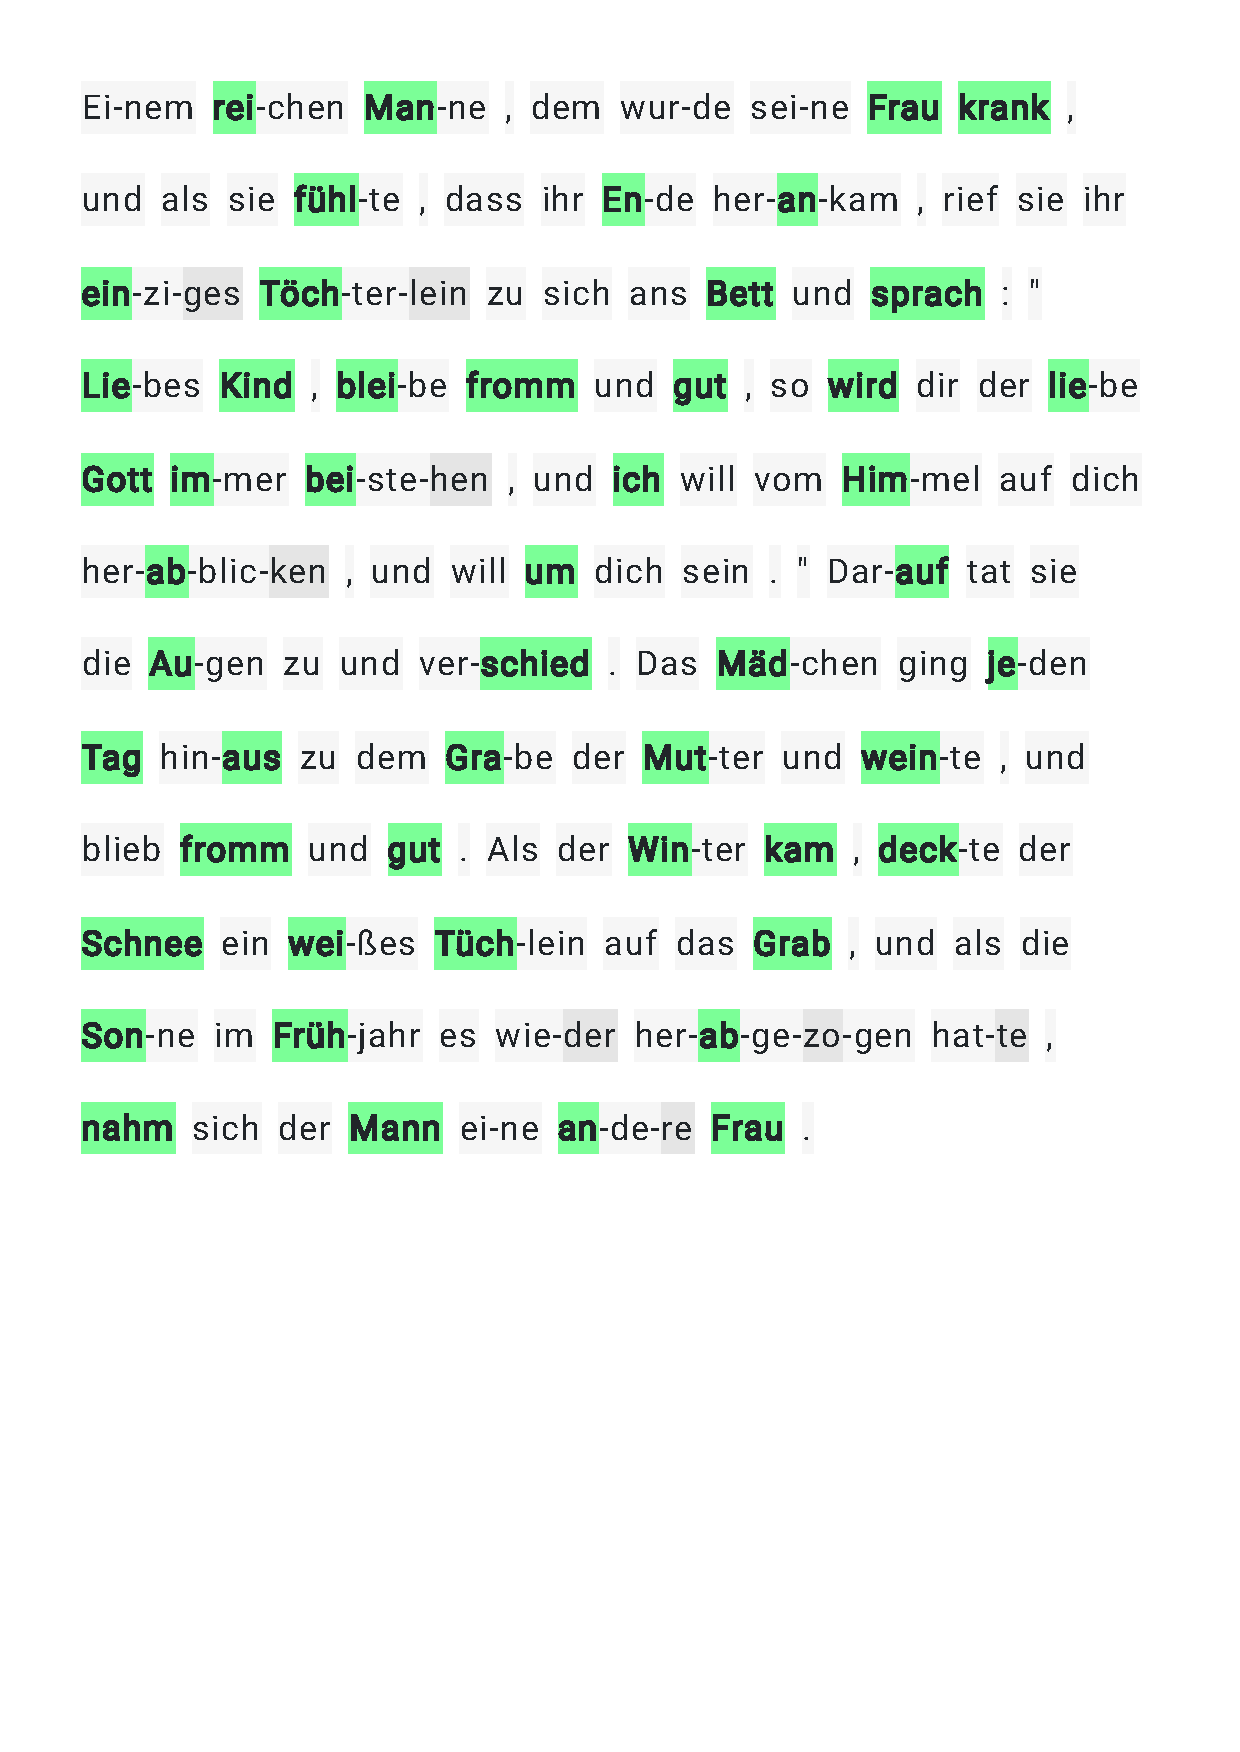
\includegraphics[width=.7\linewidth, frame]{figures/evaluation/annotation5}
	\caption{Manuelles Deaktivieren der Hervorhebung in kurzen Wörtern}
	\label{fig:evaluation-ex5}
\end{figure}
\newpage

\section{Nutzertest}

Während die Beispiele im vorherigen Abschnitt verdeutlichen, dass das Entwickelte Programm generell dazu in der Lage ist, Texte anforderungsgemäß zu annotieren, sollte der Nutzertest zeigen, dass die Applikation von der Zielgruppe (Lerntherapeuten, Nachhilfelehrer und Eltern betroffener Kinder) problemlos bedient werden kann. Intuitivität und Zeiteffizienz sollten dabei vor Allem berücksichtigt werden, da Software, die diese Kriterien schlecht erfüllt, ungern oder im schlechtesten Fall überhaupt nicht benutzt wird. \tocite{irgendwas UX}.

\subsection{Vorbereitung und Durchführung}

Der Nutzertest beinhaltete neben den statistischen Daten zu Alter und Beruf bzw. Studiengang fünf Szenarien, die der Nutzer bearbeiten sollte. Um detaillierte Informationen zur Vorgehensweise des Probanden zu erhalten, wurde im Interview mit der \textit{Thinking Aloud} Methode gearbeitet, d.h. der Proband wurde aufgefordert bei jeder Aktion, die er durchführt, möglichst genau zu beschreiben was er damit bezweckt und warum er es tut. \tocite{thinking aloud} In der schriftlichen Testbeschreibung wurde der Nutzer daher informiert, alle Arbeitsschritte der Szenarien laut vorzulesen und Kommentare und Kritik jederzeit zu äußern. Außerdem wurde in jedem Text explizit mündlich darauf hingewiesen, alle Handlungen möglichst genau zu beschreiben.\\
In der Testbeschreibung wurde auch verdeutlicht, dass es sich um ein Test des Softwaresystems handelt und nicht des Nutzers. \todo{warum wichtic, cite}\\

Um möglichst konsistente Testbedingungen zu schaffen, wurde bei allen Probanden mit einer aktuellen Version von Google Chrome gearbeitet. Es wurde zudem sichergestellt, dass den Probanden ein möglichst gewohntes Umfeld geboten wird. Im besten Fall benutzten die Nutzer ihre eigenen Computer. Falls dies nicht möglich war, wurde vorher überprüft ob beim Testgerät alles genauso wie gewohnt bedient werden konnte, d.h. Einstellungen für Peripherie wie Maus, Tastatur oder Touchpad wurden vorher, dem Nutzer entsprechend, angepasst.\\

Nach jedem der fünf Szenarien wurde von dem Proband ein After Scenario Questionnaire ausgefüllt \tocite{asq}. Es beinhaltete die folgenden drei Fragen:
\begin{itemize}
	\item \textbf{Intuitivität}: Die Aufgabe konnte ich intuitiv und problemlos erledigen.
	\item \textbf{Zeitaufwand}: Ich halte die Zeit, die ich gebraucht habe um die Aufgabe zu erledigen, für angemessen.
	\item \textbf{Dokumentation}: Ich bin mit den Informationen, die ich während der Bearbeitung in der App erhalten habe (Beschreibungen, Rückmeldungen) zufrieden.
\end{itemize}

Zustimmung oder Ablehnung der Aussagen konnte in den fünf Optionen \textit{trifft zu}, \textit{trifft eher zu}, \textit{weder noch}, \textit{trifft eher nicht zu} oder \textit{trifft nicht zu} ausgedrückt werden.

Die Software wurde insgesamt 7 Probanden getestet. Die Bedienung der Software sollte sich im besten Fall möglichst wenig unterscheiden, wenn sie durch Experten oder Laien durchgeführt wird. Daher wurden die Befragten in die entsprechenden zwei Gruppen eingeteilt. Zum einen die Expertengruppe, bestehend aus Lerntherapeuten und Nachhilfelehrern, und zum Anderen Laien, die exemplarisch für Leute aus dem Umfeld der Betroffenen stehen. Es wurden 3 Experten und 4 Laien befragt.\\

\subsection{Ergebnisse}

Im Folgenden werden die einzelnen Szenarien beschrieben und deren Ergebnisse dargestellt. Von den Probanden erkannte und während des Szenarios geäußerte Schwierigkeiten und Probleme werden tabellarisch, zusammen mit eventuellen Ansätzen zu deren Behebung dargestellt.

\subsubsection{Szenario 1: Nutzerkonto}

Zuerst sollte der Proband ein Nutzerkonto mit Mail Adresse und Passwort erstellen (hier wurde, damit der Nutzer kein sicherheitskritisches Passwort verwendet und sich das Passwort während des Tests merken kann \qq{12345678} vorgegeben). Anschließend loggt er sich ein und wieder aus.

\todo{Grafik Ergebnisse}

\begin{table}[h!]
	\centering
	\begin{tabular}{|r|l|}
		\hline
		\textbf{Problem} & \textbf{Lösungsansatz}\\
		\hline
		\hline
		problem1 & lösung1\\
		\hline
		problem1 & lösung1\\
		\hline
	\end{tabular}
	\caption{Nutzeranmerkungen zu Szenario 1}
	\label{table:szenario1}
\end{table}

\subsubsection{Szenario 2: Textanalyse}

Als nächstes loggt sich der Proband wieder ein und soll einen gegebenen Text in das Textfeld der Textanalyse kopieren und diesen dann analysieren lassen. Alle unbekannten Wörter (in der Anwendung rot hinterlegt) sollen nun manuell geklärt werden. Der Nutzer klickt so lange durch das User Interface der manuellen Analyse, bis alle Wörter annotiert sind. Als letztes soll mit den Einstellungen der Annotation experimentiert werden, bis eine Einstellung gefunden wird, die den Nutzer anspricht. Hier wurde noch mündlich hinzugefügt, dass der Nutzer, um sich damit vertraut zu machen, alle Einstellungen einmal ausprobieren sollte.

\todo{Grafik Ergebnisse}

\begin{table}[h!]
	\centering
	\begin{tabular}{|r|l|}
		\hline
		\textbf{Problem} & \textbf{Lösungsansatz}\\
		\hline
		\hline
		problem1 & lösung1\\
		\hline
		problem1 & lösung1\\
		\hline
	\end{tabular}
	\caption{Nutzeranmerkungen zu Szenario 2}
	\label{table:szenario2}
\end{table}

\subsubsection{Szenario 3: Annotationsvorlagen}

Im dritten Szenario werden dem Nutzer zweimal die erste Zeile des Textes, jeweils mit verschieden Einstellungen annotiert, gegeben. Er soll nun nacheinander versuchen, die Annotation so einzustellen, dass es so wie im gegebenen Ausschnitt aussieht. Zudem sollen diese Einstellungen als Vorlagen mit den Namen \qq{Vorlage 1} und \qq{Vorlage 2} gespeichert werden. Zum Schluss wechselt der Nutzer zwischen Vorlage 1 und Vorlage 2 hin und her.
\todo{Grafik Ergebnisse}

\begin{table}[h!]
	\centering
	\begin{tabular}{|r|l|}
		\hline
		\textbf{Problem} & \textbf{Lösungsansatz}\\
		\hline
		\hline
		problem1 & lösung1\\
		\hline
		problem1 & lösung1\\
		\hline
	\end{tabular}
	\caption{Nutzeranmerkungen zu Szenario 3}
	\label{table:szenario3}
\end{table}

\subsubsection{Szenario 4: Texte wiederverwenden}

Hier soll der Nutzer den aktuellen Text mit Titel in seinem Nutzerkonto speichern. Anschließen wird auf die Nutzerkonto Seite gewechselt und der gespeicherte Text neu analysiert.
\todo{Grafik Ergebnisse}

\begin{table}[h!]
	\centering
	\begin{tabular}{|r|l|}
		\hline
		\textbf{Problem} & \textbf{Lösungsansatz}\\
		\hline
		\hline
		problem1 & lösung1\\
		\hline
		problem1 & lösung1\\
		\hline
	\end{tabular}
	\caption{Nutzeranmerkungen zu Szenario 4}
	\label{table:szenario4}
\end{table}

\subsubsection{Szenario 5: Wort Verifizierung}

Im letzten Szenario wechselt der Nutzer auf die Verifizierungsseite. Hier sollen vier Einträge anderer Nutzer bestätigt oder verbessert verden.
\todo{Grafik Ergebnisse}

\begin{table}[h!]
	\centering
	\begin{tabular}{|r|l|}
		\hline
		\textbf{Problem} & \textbf{Lösungsansatz}\\
		\hline
		\hline
		problem1 & lösung1\\
		\hline
		problem1 & lösung1\\
		\hline
	\end{tabular}
	\caption{Nutzeranmerkungen zu Szenario 5}
	\label{table:szenario5}
\end{table}


\subsubsection{Allgemeine Anmerkungen}

Zum Schluss des Nutzertest wurde der Proband zu allgemeinen Äußerungen von Kritik und Vorschlägen zur Applikation als Ganzes aufgefordert. Wichtige Kommentare sind in der folgenden Tabelle festgehalten.

\begin{table}[h!]
	\centering
	\begin{tabular}{|r|l|}
		\hline
		\textbf{Problem} & \textbf{Lösungsansatz}\\
		\hline
		\hline
		problem1 & lösung1\\
		\hline
		problem1 & lösung1\\
		\hline
	\end{tabular}
	\caption{Allgemeine Äußerungen von Kritik und Vorschlägen}
	\label{table:usertestgeneral}
\end{table}


\section{Diskussion}

hat funktioniert\\
wurde von lerntherapeuten als nütlich bewertet, im verglich zur manuellen erstellung der texte\\
usability zeigt, das das programm grunsätzlich gut benutzbar ist, teilweise kleine änderungen nötig, damit für alle problemlos bedienbar\\
teile (wie nur eine betonung im wort) funktionieren, könnten aber noch deutlich besser gemacht/überarbeitet werden\\

einleitung aufgreifen, welche fragen, antworten dazu aus hauptteil und evaluation\\
irgendwelche fragen aus literatur beantwortet?
weitere fragen?

\section{Ausblick}

datenbank: PHONOLEX als Grundlage (statt oder zusaetzlich zu CELEX)\\
welche grundlegenden ideen können noch umgesetzt werden, wie kann die software erweitert werden?\\
...
\cleardoublepage

%% !TEX root = ../ausarbeitung.tex

\chapter{Diskussion}
Die Diskussion kann als Teil des Evaluations- oder Schlusskapitels oder als eigenständiges Kapitel aufgeführt werden. Wichtig ist, dass Sie Ihre Evaluationsergebnisse realistisch einschätzen und ins Verhältnis zum Stand der Technik setzen. Achten Sie besonders darauf, aus den Daten Ihrer Evaluation keine Wunschergebnisse abzulesen, die nicht in den Daten sind (wenn Ihre Testnutzer Ihr neuimplementiertes System nicht besser bedienen können als ein vorhandenes, dann ist das eben so). Gerade unerwartete bzw. \qq{negative} Ergebnisse (z.B. das neue System ist nicht besser als vorhandene) bringen wissenschaftliche Erkenntnisse: man stellt damit fest, dass der gewählte Weg nicht zum gewünschten Ergebnis führt und man generiert damit neue Fragen, z.B. warum der Weg nicht funktioniert hat, obwohl er vor dem Test als überlegen erachtet wurde.

Es kann auch sein, dass verschiedene Evaluationsformen Unterschiede offenbaren. Z.B. kann es sein, dass die Nutzbarkeit des implementierten Systems nicht besser ist als bei anderen Ansätzen, aber dass es deutlich einfacher zu warten ist.


Im letzten Teil runden Sie Ihre Arbeit ab, in dem Sie Ihre Argumentation aus der Einleitung aufgreifen und mit konkreten Daten aus Ihrem Hauptteil und der Evaluation untermauern. Auch hier können Sie Bezug zur Literatur nehmen. Am Ende sollten Sie einen Ausblick über weitere Forschungsthemen geben. Dabei aufpassen, dass es nicht so klingt wie \qq{mir ist die Zeit ausgegangen und folgendes habe ich nicht mehr geschafft}. Eine gute wissenschaftliche Arbeit wirft mehr Fragen auf als sie beantwortet. Es sollte also eher klingen nach \qq{meine Arbeit hat \dots gezeigt. Daraus ergeben sich weitere interessante Fragen \dots}.

\section{Ausblick}

datenbank: PHONOLEX als Grundlage (statt oder zusaetzlich zu CELEX)

%\cleardoublepage

%%% Literaturverzeichnis, lädt die Datei literatur.bib
\bibliographystyle{babplain} % "babplain" benötigt das Paket babelbib
\bibliography{library}
\cleardoublepage

%%% Selbständigkeitserklärung
\thispagestyle{empty}
\section*{Erklärung}
Hiermit erkläre ich, dass ich diese schriftliche Abschlussarbeit selbständig 
verfasst habe, keine anderen als die angegebenen Hilfsmittel und Quellen benutzt 
habe und alle wörtlich oder sinngemäß aus anderen Werken übernommenen Aussagen als 
solche gekennzeichnet habe.
\\[2cm]
Ort, Datum \hfil Unterschrift 

\end{document}